\documentclass{article}

\usepackage{fullpage}
\usepackage{parskip}
\usepackage{setspace}
\usepackage{mathtools}
\usepackage{tikz}
\usetikzlibrary{arrows}
\usetikzlibrary{decorations.markings}
\usetikzlibrary{calc}
\usepackage{standalone}
\usepackage{float}
\usepackage{caption}
\usepackage{subcaption}
\usepackage{amsmath}
\usepackage{amsfonts}
\usepackage{amsthm}
\usepackage[ruled]{algorithm2e}
\usepackage{adjustbox}
\usepackage{enumerate}
\usepackage{hyperref}
\usepackage[nocompress]{cite}


\newtheorem{definition}{Definition}
\newtheorem{theorem}{Theorem}
\newtheorem{proposition}{Proposition}
\newtheorem{lemma}{Lemma}
\newtheorem{remark}{Remark}

\title{On Deadlocking in Queueing Networks}
\author{Geraint Ian Palmer, Paul Harper, Vincent Knight}
\date{\today}


\numberwithin{equation}{section}

\begin{document}
\onehalfspacing

\maketitle

\begin{abstract}
Open restricted queueing networks give rise to the phenomenon of deadlock, that is some customers may be unable to ever leave a server due to recursive upstream blocking.
This paper explores deadlock in restricted queueing networks, presents a method of detecting deadlock in these systems, and builds Markov chain models of these deadlocking networks.
The five networks for which Markov models are given include single and multi-server networks for one and two node systems.
These models are compared to results obtained using a simulation and the above deadlock detection method.
Finally a bound on the time to deadlock of the two node single-server network with loops is derived by comparing its properties with other queueing networks that are embedded within it.
It is hoped that this paper addresses a gap in the literature on the deadlocking properties of open restricted queueing networks.

\end{abstract}

\section{Introduction \& Background}

The study and modelling of queueing networks with blocking is an important tool in many aspects of operational research, both analytically and through simulation.
These models have applications in many varied settings such as healthcare, supply chains, manufacturing and communications systems.
However, these types of models have their limitations, due to their potential to become permanently blocked in deadlock, or a deadly embrace of resources.
These deadlocks can be real in which case accurate modelling of deadlock is needed, or they can occur in models where deadlock situations are easily adjusted in reality. In the latter case, such as by swapping two customers, a good understanding of deadlock is needed in order to model the adjusted reality.

Figure~\ref{fig:1st_example} shows an open two node restricted queueing network in deadlock.
The customer at the top server is blocked from entering the bottom node as there is a full queue, and similarly the customer at the bottom server is blocked from entering the top node as there is a full queue.
It is clear that by following the rules of a queueing network, no more natural movement can happen.

\begin{figure}[!htbp]
  \begin{center}
  \includestandalone[width=0.3\textwidth]{images/2nodesindeadlock}
  \end{center}
  \caption{Example of an open two node restricted queueing network in deadlock.}
  \label{fig:1st_example}
\end{figure}

Restricted open queueing networks that can experience deadlock are under-discussed in the literature.
This paper aims to explore deadlock to gain this understanding in order to build more accurate models of deadlocking systems

This paper is structured as follows: the remainder of this section sets up the
notation and definitions used for the rest of the paper.
Section~\ref{sec:litreview} discusses the existing literature on deadlock in
queueing networks. Section~\ref{sec:detectingdeadlock} presents a method of
detecting deadlock in simulations of queueing networks.
Section~\ref{sec:simulation} briefly describes the discrete event simulation
model used to obtain the results in this paper. Section~\ref{sec:markovmodels}
presents Markov models of five deadlocking queueing networks, derives their
expected time to deadlock, and compares these with results obtained through the
simulation model. Finally Section~\ref{sec:bound} derives a bound for the
expected time to deadlock for one of the queueing networks discussed.

\subsection{Open Restricted Queueing Networks}

Queueing networks are described as open if customers can enter and leave the
system from outside of the system.
Restricted networks are those where at least one service centre has limited queueing space or capacity before it.

This paper is concerned with open restricted queueing networks that experience
so called Type I blocking, which will be defined in Section X.
% I don't care how you spell centre (US), center (UK) but just check that you're
% consistent throughout
Throughout this paper service centers will be referred to as nodes, and for the $i$th node of an open restricted queueing network the following notation is used:

\begin{itemize}
  \item $\Lambda_i$ denotes the external arrival rate.
  \item $\mu_i$ denotes the service rate.
  \item $c_i$ denotes the number of parallel servers.
  \item $n_i$ denotes the queueing capacity.
  \item $r_{ij}$ denotes the routing probability from node $i$ to node $j$ upon completion of service at node $i$.
\end{itemize}

Exponential service times and Poisson arrivals are assumed.

For the purposes of this paper, deadlock is defined as follows.\\

\begin{definition}
    When a queueing network is in a state where at least one service
    station ceases to begin or finish any more services due to
    recursive upstream blocking, the system is said to be in deadlock.
\end{definition}

In the next section a review of the current literature on deadlock is given.


\section{Literature Review}\label{sec:litreview}


Restricted queueing networks that exhibit blocking are well discussed in the literature, both exact \cite{hunt56, baber08, aviitzhakyadin65, koizumietal05, latoucheneuts80, perrosetal88} and approximate methods \cite{takahashi80, korporaaletal00, onvural90, perrosetal88}. Discussion on restricted queueing networks with feedback loops, that may exhibit deadlock, are sparse however.
In fact, the problem of deadlock in queueing networks has either been ignored, not studied, or assumed resolved in much of the literature \cite{onvural90, perrosetal88}.

Central to the study of deadlock in queueing networks is the concept of blocking.
In \cite{onvuralperros86} three types of blocking are described:

\begin{itemize}
    \item Type I blocking (blocked at service, BAS, transfer blocking) occurs when a customer is blocked after completing service, and remains with the server until capacity at their destination node becomes available.
    \item Type II blocking (blocked before service, BBS, service blocking) occurs when a customer declares their destination before beginning service, and is only granted service if there is available capacity at their destination node.
    \item In Type III blocking (repetitive services, RS-FD and RS-RD, rejection blocking) instead of getting blocked a customer is required to repeat their service if there is no capacity at their destination. This type of blocking comes in two flavours, fixed destination where the customer's destination does not change at each repetition of service, and random destination, where the customer's destination is re sampled from a probability distribution after each repetition.
\end{itemize}

There has been a lot of research into detection and prevention of deadlock which doesn't consider the underlying stochastic structure of the system \cite{coffmanelphick71}.
These general deadlocks occur in flexible manufacturing systems and distributed communication systems.
Conditions for this type of deadlock, also referred to as deadly embraces \cite{coffmanelphick71}, to potentially occur are given:
\begin{itemize}
  \item Mutual exclusion: Tasks have exclusive control over resources.
  \item Wait for: Tasks do not release resources while waiting for other resources.
  \item No preemption: Resources cannot be removed until they have been used to completion.
  \item Circular wait: A circular chain of tasks exists, where each task requests a resource from another task in the chain.
\end{itemize}

In open restricted queueing networks the mutual exclusion condition is satisfied as customers cannot share servers; the wait for condition is satisfied due to the blocking rules defined previously; the no preemption condition is satisfied in networks that have no or non-preemptive priority (this report will only look at networks with no priority); and the circular wait condition is satisfied if the queueing network contains a cycle where all nodes have limited queueing capacity, that is feedback loops.

Allowing a system to reach deadlock can be problamatic in cases where automated systems cannot continue operations, or where simulations cannot accurately model reality.
In general there are three strategies for dealing with the problem of deadlock \cite{kawadkaretal14, elmagarmid86}:

\begin{itemize}
  \item Prevention, in which the system cannot possibly deadlock in the first place.
  \item Avoidance, in which decisions are made as time unfolds to avoid reaching deadlock.
  \item Detection and recovery.
\end{itemize}

The third of these, detection and recovery, will be discussed in this paper, although a brief overview of the others is also given.

\subsection{Deadlock Prevention}

Deadlock prevention has been discussed in queueing networks under Type I blocking.
For closed networks of $K$ customers with only one class of customer, \cite{kunduakyildiz89} proves the following condition to ensures no deadlock: for each minimum cycle $C$, $K < \sum_{j\in C} B_j$, the total number of customers cannot exceed the total queueing capacity of each minimum subcycle of the network.
The paper also presents algorithms for finding the minimum queueing space required to ensure deadlock never occurs for closed cactus networks, where no two cycles have more than one node in common.
This result is extended to multiple classes of customer in \cite{liebeherrakyildiz95}, with more restrictions such as single servers and each class having the same service time distribution.
Here a integer linear program is formulated to find the minimum queueing space assignment that prevents deadlock.

Further conditions on deadlock prvention in closed queueing networks are reviewed in \cite{onvural90}, including closed networks under different blocking mechanisms such Type II and Type III blocking.
The literature does not discuss deadlock properties in open restricted queueing networks.


\subsection{Deadlock Avoidance}

There are algorithms discussed in the literature for the dynamic avoidance of deadlock.
In the Banker's Algorithm \cite{dijkstra82, kawadkaretal14}, unsafe states, those that will lead to deadlock, are avoided by ensuring actions leading to these states are not carried out.

A common deadlock avoidance technique in flexible manufacturing systems is the use of dynamic resource allocation policies using petri net nodels of the system \cite{viswanadhametal90, ezpeletaetal02}.
Some resource allocations are disallowed if that allocaton will lead to deadlock.

Another deadlock avoidance algorithm in \cite{belik90}, for systems with one type of each resource, makes use of a directed resource allocation graph. Resource requests are not allocated resources if that allocation leads to a directed cycle in the resource allocation graph.

\subsection{Deadlock Detection \& Recovery}

A popular method of detecting general deadlock is the use of wait-for graphs, state-graphs and their variants \cite{cheng90, elmagarmid86, coffmanelphick71, choetal95}.
These wait-for graphs, keep track of all circular wait relations between tasks.

In \cite{coffmanelphick71} dynamic state-graphs are defined with resources as vertices and requests as edges.
For scenarios where there is only one type of each resource, deadlock arises if and only if the state-graph contains a cycle.
In \cite{choetal95} the vertices and edges of the state graph are given labels in relation to a reference node.
Using these labels \textit{simple bounded circuits} are defined whose existence within the state graph is sufficient to detect deadlock.
This type of strategy is used in this paper to detect deadlock in queueing systems.

Deadlock detection and recovery in closed queueing networks through swapping customers is assumed in \cite{perrosetal88}, with zero transition time assumed between deadlocked states and the corresponding resolved state. Though time to resole deadlock may not be negligible in reality.
In \cite{akyildiz89}, deadlock detection and recovery is listed as one of the two possible solutions for handling deadlock in queueing networks, although this isn't discussed further.

The next section introduces a method of detecting when deadlock occurs in open restricted queueing networks.

\section{Deadlock Detection}\label{sec:detectingdeadlock}

In order to detect when deadlock has occured in a queueing network simulation, the state digraph is used.
This is a form of wait-for graph, and is defined below.\\

\begin{definition}
The state digraph $D(t)$ of a queueing network defines that network's state at any time $t$.
Vertices of the state digraph correspond to servers of the network.
A directed edge denotes a blockage relationship in the following manner: if a customer at the $k$th server of node $i$ is blocked from entering node $j$, then there are directed edges from the vertex corresponding to node $i$'s $k$th server to every vertex corresponding to the servers of node $j$.
\end{definition}

To illustrate this concept Figure~\ref{fig:exampledigraphs} show examples of queueing network in and out of deadlock, and the corresponding state digraph in each case.

\begin{figure}[!htbp]
\begin{center}
  \begin{subfigure}{0.45\textwidth}
    \begin{center}
      \includestandalone[width=0.8\textwidth]{images/exampledigraph_1}
    \end{center}
    \caption{A three node queueing network in deadlock, with state digraph.}
    \label{fig:exampledigraph_deadlock}
  \end{subfigure}
  \hspace{6 mm}
  \begin{subfigure}{0.45\textwidth}
    \begin{center}
      \includestandalone[width=0.8\textwidth]{images/exampledigraph_2}
    \end{center}
    \caption{A three node queueing network not in deadlock, with state digraph.}
    \label{fig:exampledigraph_nodeadlock}
    \vspace{6 mm}
  \end{subfigure}
  \begin{subfigure}{0.45\textwidth}
    \begin{center}
      \includestandalone[width=0.9\textwidth]{images/exampledigraph_3}
    \end{center}
    \caption{A three node queueing network in not deadlock, with state digraph.}
    \label{fig:exampledigraph_nodeadlock}
  \end{subfigure}
  \hspace{6 mm}
  \begin{subfigure}{0.45\textwidth}
    \begin{center}
      \includestandalone[width=0.9\textwidth]{images/exampledigraph_4}
    \end{center}
    \caption{A three node queueing network in deadlock, with state digraph.}
    \label{fig:exampledigraph_nodeadlock}
    \vspace{6 mm}
  \end{subfigure}
  \end{center}
  \caption{Examples of state digraphs with their corresponding queueing networks.}
  \label{fig:exampledigraphs}
\end{figure}

Consider one weakly connected component $G(t)$ of $D(t)$. Consider the node $X \in G(t)$. Some observations:

\begin{itemize}

  \item If $X$ is unoccupied, then $X$ has no incident edges.
  \item Consider the case when $X$ is occupied by individual $a$, whose next destination is node $j$. Then $X$'s direct successors are the servers occupied by individuals who are blocked or in service at node $j$.
  \item It can interpreted that all $X$'s descendants are the servers whose occupants are directly or indirectly blocking $a$, and interpret all $X$'s ancestors as those servers whose individuals who are being blocked directly or indirectly by $a$.
  \item All vertices of $G(t)$ are either descendants of another vertex and so are occupied by an individual who is blocking someone; or are ancestors of another vertex, and so are occupied by someone who is blocked.
  \item Note that the only possibilities for $\text{deg}^{\text{out}}(X)$ are 0 or $c_j$. If $\text{deg}^{\text{out}}(X) = c_j$ then $a$ is blocked by all its direct successors. The only other situation is that $a$ is not blocked, and $X \in G(t)$ because $a$ is in service at $X$ and blocking other individuals, in which case $\text{deg}^{\text{out}}(X) = 0$.
  \item It is clear that if all of $X$'s descendants are occupied by blocked individuals, then the system is deadlocked at time $t$.
  \item By definition all of $X$'s ancestors are occupied by blocked individuals.

\end{itemize}

The following results detect deadlock for open restricted queueing networks.\\

\begin{theorem}
A deadlocked state arises at time $t$ if and only if $D(t)$ contains a knot.
\end{theorem}

\begin{proof}
Consider one weakly connected component $G(t)$ of $D(t)$ at time $t$.

Assume that $G(t)$ contains a vertex $X$ such that $\text{deg}^{\text{out}}(X) = 0$, and there is a path from every other non-sink vertex to $X$.
This implies that $X$'s occupant is not blocked and is a descendant of another vertex.
Therefore $Q$ is not deadlocked as there does not exist a vertex whose descendants are all blocked.

Now assume that we have deadlock.
For a vertex $X$ who is deadlocked, all descendants of $X$ are are occupied by individuals who are blocked, and so must have out-degrees greater than 0.
And so there is no path from $X$ to a vertex with out-degree of 0.

\end{proof}

The knot condition can be simplified for specific cases.\\

\begin{proposition}
For queueing networks:
\begin{enumerate}
  \item with one node
  \item with two nodes, each with two or fewer parallel servers
  \item with a finite amount of nodes, each with a single-server
\end{enumerate}
a deadlocked state arises if and only if there exists a weakly connected component without a sink node.
\end{proposition}

\begin{proof}

\begin{enumerate}

\item
Consider a one node queueing network.

If there is deadlock, then all servers are occupied by blocked individuals, and so all servers have an out-edge.

\item
Consider a two node queueing network, each node with 2 or fewer parallel servers.

If both nodes are involved in the deadlock, so there is a customer in node 1 blocked from entering node 2, and a customer from node 2 blocked from entering node 1, then all servers in node 1 and node 2 in $D(t)$ will have out edges as they are occupied by a blocked individual.
The servers of node 1 and 2 consist of the entirety of $D(t)$, and so there is no sink nodes.

Now consider the case when only one node is involved in the deadlock.
Without loss of generality, let's say that node 1 is in deadlock with itself, then the servers of node 1 have out-edges.
For the servers of node 2 to be part of that weakly connected component, there either needs to be an edge from a server in node 1 to a server in node 2, or an edge from a server in node 2 to a server in node 1.
An edge from a server in node 1 to a server in node 2 implies that a customer from node 1 is blocked from entering node 2, and so node 1 is not in deadlock with itself.
An edge from a server in node 2 to a server in node 1 implies that a customer in node 2 is blocked from entering node 1.
In this case one server in node 2 has an out-edge.
Now either the other server of node two is empty or still in service, and so isn't part of that weakly connected component, or the other server's customer is blocked and so has an out edge.

For the case of a two node queueing network with at least one node with more than 2 servers, consider the following counter-example:

Node $A$ has two parallel server, node $B$ has three parallel sevrers.
Begin with all servers occupied by customers in service and full queues.
The customer at server $A_1$ is blocked to node $A$.
The customer at server $B_1$ is blocked to node $A$.
The customer at server $B_2$ is blocked to node $B$.
The customer at server $A_2$ is blockec to node $A$.
The resulting state digraph in Figure~\ref{fig:counter_example_1} has a weakly connected component with a sink.

\item
Consider a queueing network with $N$ nodes, each with a single-server.

If $1 \leq n \leq N$ nodes are involved in the deadlock, then each server in those $n$ nodes has a blocked customer, and so has an out-edge.
Of the other nodes, they can only be in the same weakly connected component if either they contain a indiviual blocked by those in deadlock, in which case they will have an out edge; or they contain a blocked individual blocked by those directly or indirectly blocked by those in deadlock, in which case they will have an out edge; or they are blocking someone who is blocked directly or indirectly by those in deadlock.
However this last case cannot happen, as every node is single-server each person can only be blocked by one other individual at a time.

For the case of a queueing network with more than two nodes with multiple servers, the following counter-example proves the claim:

Node $A$ has one parallel server, node $B$ has two parallel servers, and node $C$ has three parallel servers.
Begin with all servers occupied by customers in service and full queues.
The customer at server $B_1$ is blocked from entering node $A$.
Then the customer at server $C_1$ is blocked from entering node $B$.
Then the customer at server $A_1$ is blocked from entering node $A$.
The resulting state digraph in Figure~\ref{fig:counter_example_2} has a weakly connected component with a sink.
\end{enumerate}
\end{proof}

\begin{figure}
\begin{subfigure}{0.5\textwidth}
\begin{center}
\includestandalone[width=0.8\textwidth]{images/counter_example_digraph_1}
\end{center}
\caption{State Digraph of Counter-Example 1.}
\label{fig:counter_example_1}
\end{subfigure}
\begin{subfigure}{0.5\textwidth}
\begin{center}
\includestandalone[width=0.65\textwidth]{images/counter_example_digraph_2}
\end{center}
\caption{State Digraph of Counter-Example 2.}
\label{fig:counter_example_2}
\end{subfigure}
\caption{Counter examples.}
\label{fig:counter_examples}
\end{figure}

The next section briefly discusses the simulation model used to conduct numerical experiments for this paper.









\section{Simulation Model}\label{sec:simulation}

A simulation model is used to run a discrete event simulation of the open restricted queueing network, detect deadlock and stop the simulation at this point.
The time the simulation ran for until deadlock is recorded.
The model is generic, and can handle any number of service center nodes, each defined by its external arrival rate, service rate, number of servers and queueing capacity, which may be set to $\infty$ is needed.
A routing matrix with entries $r_{ij}$ describes how every node is connected to every other node.

The simulation model is built in an object-orientated manor using Python.
Customers, nodes, servers and the queueing network itself are objects that interact or contain each other.
A dummy arrival node and exit node exist to spawn customers and collect data.
The code for the simulation can be found here: \url{https://github.com/geraintpalmer/QNetSim}.

The main simulation loop is carried out as follows:

\begin{algorithm}[H]
    \DontPrintSemicolon
    Find next active node\;
    \While{not deadlocked}{
        Next active node has event\;
        \For{all nodes}{
            update next event date\;
        }
        detect deadlock\;
        \If{deadlocked}{
            record current time\;
        }
        next active node $\leftarrow$ node with closest next event date\;
        current time $\leftarrow$ next event date of next active node\;
    }
\end{algorithm}

Where each node has a `have event' subroutine.
The arrival node's `have event' subroutine creates a new customer and sends that customer to their correct starting node.
The exit node has no `have event' subroutine.
All other nodes' `have event' subroutine occurs when a customer finishes service at that node, and is carried out as follows:

\begin{algorithm}[H]
    \DontPrintSemicolon
    Identify customer finishing service\;
    Identify customer's destination node\;
    \eIf{destination node has spare capacity}{
        Send customer to destination node\;
        \If{Customer able to start service at destination}{
            Start service
        }
        \If{Customer at front of queue can start service}{
            Start service
        }
        \If{Blocked individuals waiting to enter}{
            Unblock and accept blocked individual
        }
    }{
        Block individual
    }
\end{algorithm}

The state digraph $D(t)$ described in Section~\ref{sec:detectingdeadlock} is an attribute of the queueing network.
Edges are created or removed whenever the following events take place: a customer begins service at a server, a customer becomes blocked, a customer leaves a server.
The model is a discrete event simulation, and the deadlocked condition is checked immediately before the clock is moved on.
Here a brute force algorithm is used to check whether each strongly connected component of $D(t)$ is a knot.
Once a knot is found the simulation terminates and the time elapsed recorded.


The next section builds Markov models of five queueing networks, and discusses their deadlocking properties.










\section{Markovian Models of Deadlocking Queueing Networks}\label{sec:markovmodels}

In this section markov models are build for the following deadlocking queueing networks, and their expected time to deadlock found:

\begin{itemize}
  \item Open one node, single-server restricted queueing network with feedback loop. (Section~\ref{sec:1nodenet})
  \item Open two node, single-server restricted queueing network with routes between nodes. (Section~\ref{sec:2nodewithoutselfloops})
  \item Open two node, single-server restricted queueing network with routes between nodes and feedback loops. (Section~\ref{sec:2nodeselfloops})
  \item Open one node, multi-server restricted queueing network with feedback loop. (Section~\ref{sec:1nodeMS})
  \item Open two node, mutli server restricted queueing network with routes between nodes. (Section~\ref{sec:2nodeMS})
\end{itemize}

In general a continuous Markov chain model of a deadlocking queueing network is a set of states $s \in S$ and the transition rates between these states $q_{s_1,s_2}$.
Each state $s$ uniquely defines a configuration of customers around the queueing network.
Deadlocked states are also present, either denoted by that specific configuration of customers, or by negative numbers, for example $-1$.
Deadlocked states cannot transition to any other state, and so are absorbing states of the Markov chain.
Therefore any queueing network that can experience deadlock is guaranteed to experience deadlock, as absorbing Markov chains are guaranteed to enter one of its absorbing states.

The expected time until deadlock is reached is equivalent to the expected time to absorbtion of the Markov chain, which can easily be found \cite{stewart09}.
The canonical form of an absorbing Markov chain is

\begin{equation*}
P = \left(\begin{matrix} T & U\\ 0 & I \end{matrix} \right)
\end{equation*}

where $I$ is the identity matrix.

Now the expected number of time steps until absorption starting from state $i$ is the $i\text{th}$ element of the vector

\begin{equation} \label{eq:abs_probs}
  (I - T)^{-1}e
\end{equation}

where $e$ is a vector of 1s.

Therefore by discretising the continuous Markov chain and ensuring the correct order of states, the expected number of time steps to absorption, or deadlock can be found.

When there is more than one deadlocked state, there is more than one absorbing state in the Markov chain.
Here the expected time to absorbtion is the expected time to a deadlocked state, whichever one that may be.
The probabilities of which absorbing state a Markov chain will reach are given by the $(i, j)^{\text{th}}$ element of the vector
\begin{equation}
  (I - T)^{-1}U
\end{equation}

which corresponds to the probability of reaching absorbing state $j$ from transient state $i$.









\subsection{One Node Single-Server}\label{sec:1nodenet}

Consider the open one node single-server restricted queueing network with feedback loop shown in Figure~\ref{fig:queueingnetwork_1node}.
This shows an \(M/M/1/n\) queue where customers arrive at a rate of $\Lambda$ and served at a rate $\mu$.
Once a customer has finished service they rejoin the queue with probability $r_{11}$, and so exit the system with probability $1 - r_{11}$.

Let this system be denoted by $\Omega_1$ with parameter set $(\Lambda$, $\mu$, $n$, $r_{11})$, and the time to deadlock of this system be denoted by $\omega_1$.

\begin{figure}[!htbp]
  \begin{center}
  \includestandalone[width=0.75\textwidth]{images/1nodeexample}
  \end{center}
  \caption{An open one node single-server restricted queueing network.}
  \label{fig:queueingnetwork_1node}
\end{figure}

State space:
        \[S = \{i\in\mathbb{N} \nonscript\; | \nonscript\; 0 \leq i \leq n + 1
        \}\cup\{(-1)\}\]
where \(i\) denotes the number of individuals in service or waiting, and $(-1)$ denotes the deadlocked state.

Define $\delta = i_2 - i_1$ for all $i_k \geq 0$. The transitions are given by:

\begin{equation}
  q_{i_1, i_2} = \left\{
  \begin{matrix*}[ r ]
    \left. \begin{matrix*}[ r ]
      \Lambda & \text{if } i_1 < n + 1 \\
      0 & \text{otherwise}
    \end{matrix*} \right\} & \text{if } \delta = 1 \\
    (1 - r_{11})\mu & \text{if } \delta = -1 \\
    0 & \text{otherwise}
  \end{matrix*} \right.
\end{equation}

\begin{equation}
  q_{i, (-1)} = \left\{
  \begin{matrix*}[ r ]
    r_{11}\mu & \text{if } i = n + 1 \\
    0 & \text{otherwise}
  \end{matrix*}
  \right.
\end{equation}

\begin{equation}
  q_{-1, i} = 0
\end{equation}

The Markov chain is shown in Figure~\ref{fig:1nodeMC}.

\begin{figure}[!htbp]
  \begin{center}
    \includestandalone[width=0.75\textwidth]{images/markov_chain_1node}
  \end{center}
  \caption{Diagrammatic representation of the Markov chain for $\Omega_1$.}
  \label{fig:1nodeMC}
\end{figure}

Figure~\ref{fig:timestodeadlock} shows the effect of varying the parameters of the queueing network on times to deadlock.
Base parameters of $\Lambda = 10$, $n = 3$, $\mu = 5$ and $r_{11} = 0.25$ are used.

It can be seen that increasing the arrival rate $\Lambda$ and the transition probability $r_{11}$ results in reaching deadlock faster.
This is intuitive as increasing these parameters results in the queue filling up quicker.
Increasing the queueing capacity $n$ results in reaching deadlock slower.
Again this is intuitive, as increasing the queueing capacity allows more customers in the system before becoming deadlocked.


\begin{figure}[!htbp]
\begin{center}
\begin{subfigure}[b]{0.35\textwidth}
  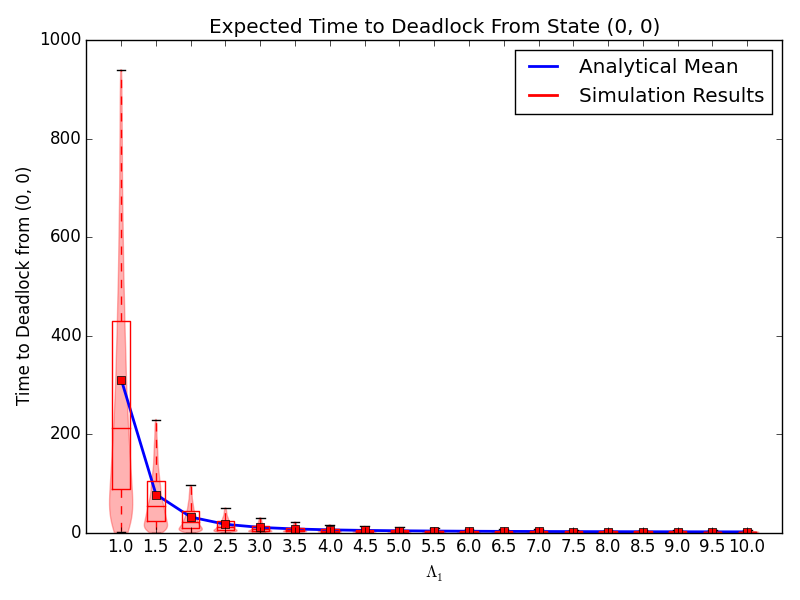
\includegraphics[width=\textwidth]{images/varyL}
  \caption{Varying $\Lambda$}
  \label{fig:timestodeadlock_L}
\end{subfigure}
\begin{subfigure}[b]{0.35\textwidth}
  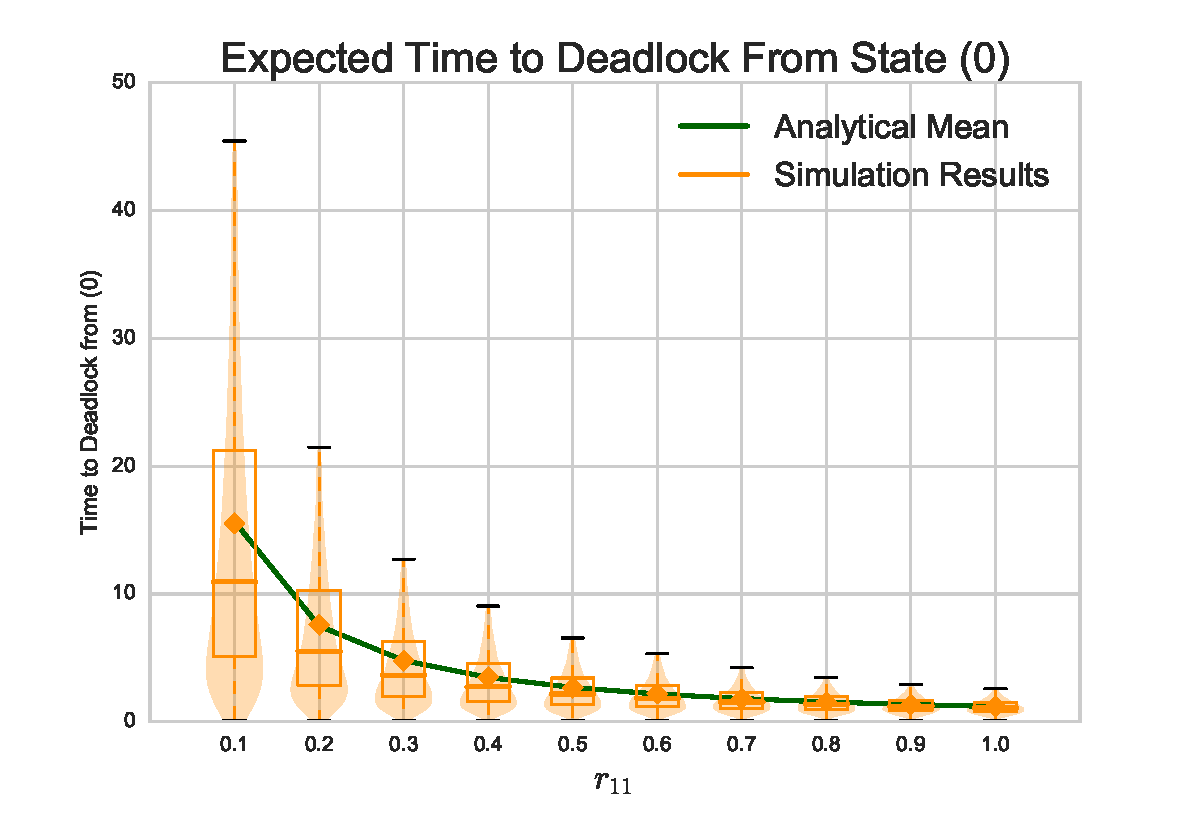
\includegraphics[width=\textwidth]{images/varyr11}
  \caption{Varying $r_{11}$}
  \label{fig:timestodeadlock_r11}
\end{subfigure}\\
\begin{subfigure}[b]{0.35\textwidth}
  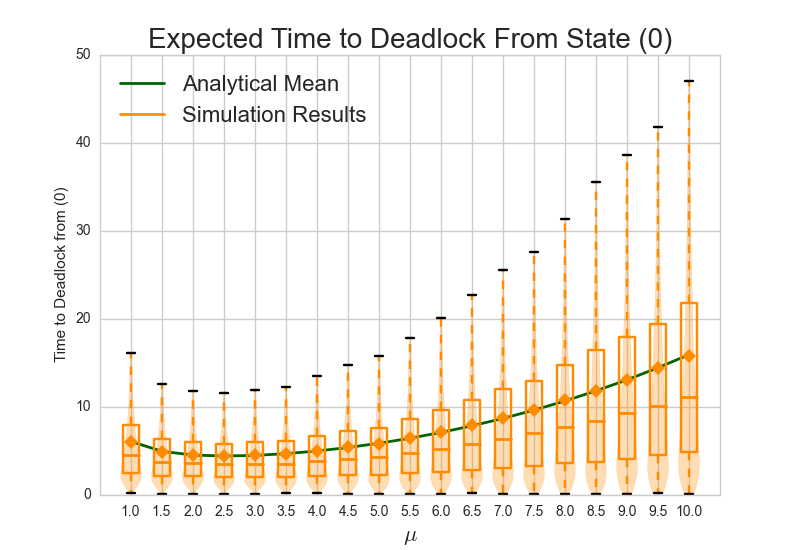
\includegraphics[width=\textwidth]{images/varymu}
  \caption{Varying $\mu$}
  \label{fig:timestodeadlock_mu}
\end{subfigure}
\begin{subfigure}[b]{0.35\textwidth}
  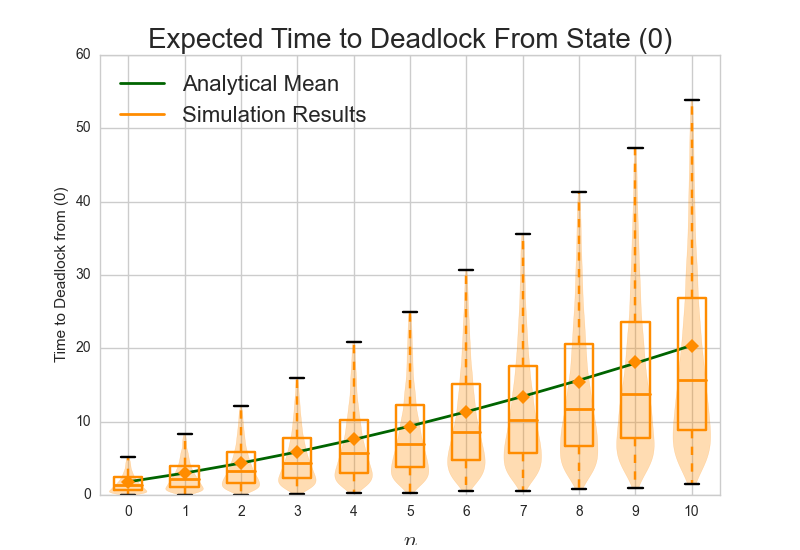
\includegraphics[width=\textwidth]{images/varyn}
  \caption{Varying $n$}
  \label{fig:timestodeadlock_n}
\end{subfigure}
\end{center}
\caption{Time to deadlock in $\Omega_1$, analytical \& simulation results (10,000 iterations).}
\label{fig:timestodeadlock}
\end{figure}

The behaviour as the service rate $\mu$ varies is not monotonic, as the service rate contributes towards both moving customers from the system and allowing customers to rejoin the queue, causing blockages and deadlock.
This behaviour is described in the following remark.\\

\begin{remark}\label{rem:oneminima}
The function $\omega_1(\mu)$ that describes the time to deadlock of an $\Omega_1$ system as the service rate $\mu$ varies, and all other parameters are fixed, has one critical point and is a local minimum for $\mu \in (0, \infty)$.
\end{remark}

The behaviour of $\omega_1(\mu)$ can be interpreted as follows:
\begin{itemize}
\item At $\lim_{\mu \to 0} \omega_1 (\mu)$ there is infinite service time, and so infinite time until deadlock.
\item At $\lim_{\mu \to \infty} \omega_1 (\mu)$ there is zero service time, the queue can never fill up, and so infinite time to deadlock.
\item At low service rates below a certain threshold $\hat{\mu}$, the arrival rate is relatively large compared to the service rate, and we can assume a saturated system.
At this point services where a customer exits the system does not have much of an effect, as we can assume another arrival immediately.
However services where a customer wishes to rejoin the queue results in a blockage as the system is saturated.
Therefore, increasing the service rate here increases the chance of a blockage, and so the chance of deadlock.
\item Above $\hat{\mu}$ the service rate is large enough that we cannot assume a saturated system, and so services where the customer exits the system does have an affect on the number of customers in the system.
Thus increasing the service rate removes people from the system, and as such there is less chance of getting blocked and deadlocked.
\end{itemize}

\begin{remark}\label{rem:findmaximum}
$\arg\max_{\mu \in [a, b]} \omega_1(\mu)$ is either $a$ or $b$.

From the closed interval method of finding absolute maximum \cite{tan09}, the absolute maximum of $\omega_1(\mu)$ on the closed interal $[a, b]$ is either the critical points in $(a, b)$, $a$ or $b$.
The only critical point in $(a, b)$ is $\hat{\mu}$, and is a local minimum (from Remark~\ref{rem:oneminima}), and so $\hat{\mu} \leq a$ and $\hat{\mu} \leq b$.
Therefore $\omega_1(\mu)$ obtains its maximum at either $a$ or $b$.
\end{remark}











\subsection{Two Node Single-Server without Self-Loops}\label{sec:2nodewithoutselfloops}

Consider the open two node single-server restricted queueing network shown in Figure~\ref{fig:queueingnetwork_2nodes}.
This shows two \(M/M/1/n_i\) queues, with service rates $\mu_i$ and external arrival rates $\Lambda_i$.
All routing possibilities $r_{ij}$ are possible except self-loops $r_{ii}$ for each node $i$.

Let this system be denoted by $\Omega_2$ with parameter set $(\Lambda_1$, $\Lambda_2$, $\mu_1$, $\mu_2$, $n_1$, $n_2$, $r_{12}$, $r_{21})$.

\begin{figure}[!htbp]
  \begin{center}
  \includestandalone[width=0.75\textwidth]{images/2nodeexample}
  \end{center}
  \caption{An open two node single-server restricted queueing network.}
  \label{fig:queueingnetwork_2nodes}
\end{figure}

State space:
    \[S = \{(i,j)\in\mathbb{N}^{(n_1+2\times n_2+2)} \nonscript\; | \nonscript\; 0 \leq i + j \leq n_1 + n_2 + 2
    \}\cup\{(-1)\}\]

    where \(i\) denotes the number of individuals:
        \begin{itemize}
            \item In service or waiting at the first node.
            \item Occupying a server but having finished service at the
                second node waiting to join the first.
        \end{itemize}
    where \(j\) denotes the number of individuals:
        \begin{itemize}
            \item In service or waiting at the second node.
            \item Occupying a server but having finished service at the
                first node waiting to join the second.
        \end{itemize}
    and the state $(-1)$ denotes the deadlocked state.

Define $\delta = (i_2, j_2) - (i_1, j_1)$ for all $(i_k, j_k) \in S$. The transitions are given by:

\begin{equation}
  q_{(i_1, j_1),(i_2, j_2)} = \left\{
  \begin{matrix*}[ r ]
    \left. \begin{matrix*}[ r ]
      \Lambda_1 & \text{if } i_1 < n_1 + 1 \\
      0 & \text{otherwise}
    \end{matrix*} \right\} & \text{if } \delta = (1, 0) \\
    \left. \begin{matrix*}[ r ]
      \Lambda_2 & \text{if } j_1 < n_2 + 1 \\
      0 & \text{otherwise}
    \end{matrix*} \right\} & \text{if } \delta = (0, 1) \\
    \left. \begin{matrix*}[ r ]
      (1 - r_{12})\mu_1 & \text{if } j_1 < n_2 + 2 \\
      0 & \text{otherwise}
    \end{matrix*} \right\} & \text{if } \delta = (-1, 0) \\
    \left. \begin{matrix*}[ r ]
      (1 - r_{21})\mu_2 & \text{if } i_1 < n_1 + 2 \\
      0 & \text{otherwise}
    \end{matrix*} \right\} & \text{if } \delta = (0, -1) \\
    \left. \begin{matrix*}[ r ]
      r_{12}\mu_1 & \text{if } j_1 < n_2 + 2 \text{ and } (i_1, j_1) \neq (n_1 + 2, n_2) \\
      0 & \text{otherwise}
    \end{matrix*} \right\} & \text{if } \delta = (-1, 1) \\
    \left. \begin{matrix*}[ r ]
      r_{21}\mu_2 & \text{if } i_1 < n_1 + 2 \text{ and } (i_1, j_1) \neq (n_1, n_2 + 2) \\
      0 & \text{otherwise}
    \end{matrix*} \right\} & \text{if } \delta = (1, -1) \\
    0 & \text{otherwise}
  \end{matrix*} \right.
\end{equation}

\begin{equation}
  q_{(i_1, j_1), (-1)} = \left\{
  \begin{matrix*}[ r ]
    r_{21}\mu_2 & \text{if } (i, j) = (n_1, n_2 + 2) \\
    r_{12}\mu_1 & \text{if } (i, j) = (n_1 + 2, n_2) \\
    0 & \text{otherwise}
  \end{matrix*}
  \right.
\end{equation}

\begin{equation}
  q_{-1, s} = 0
\end{equation}

For $n_1 = 1$ and $n_2 = 2$, the resulting Markov chain is shown in Figure~\ref{fig:2nodeMC}.

\begin{figure}[!htbp]
    \begin{center}
    \includestandalone[width=0.75\textwidth]{images/markov_chain}
    \end{center}
    \caption{Diagrammatic representation of the Markov chain for $\Omega_2$ with $n_1=1$ and $n_2=2$.}
    \label{fig:2nodeMC}
\end{figure}

Figure~\ref{fig:timestodeadlock2} shows the effect of varying the parameters of the above Markov model.
Base parameters of $\Lambda_1 = 4$, $\Lambda_2 = 5$, $n_1 = 3$, $n_2 = 2$, $\mu_1 = 10$, $\mu_2 = 8$, $r_{12} = 0.25$ and $r_{21} = 0.15$ are used.
Similar behaviour to Figure~\ref{fig:timestodeadlock} can be seen.

\begin{center}
\begin{figure}[!htbp]
\begin{center}
\begin{subfigure}[b]{0.38\textwidth}
  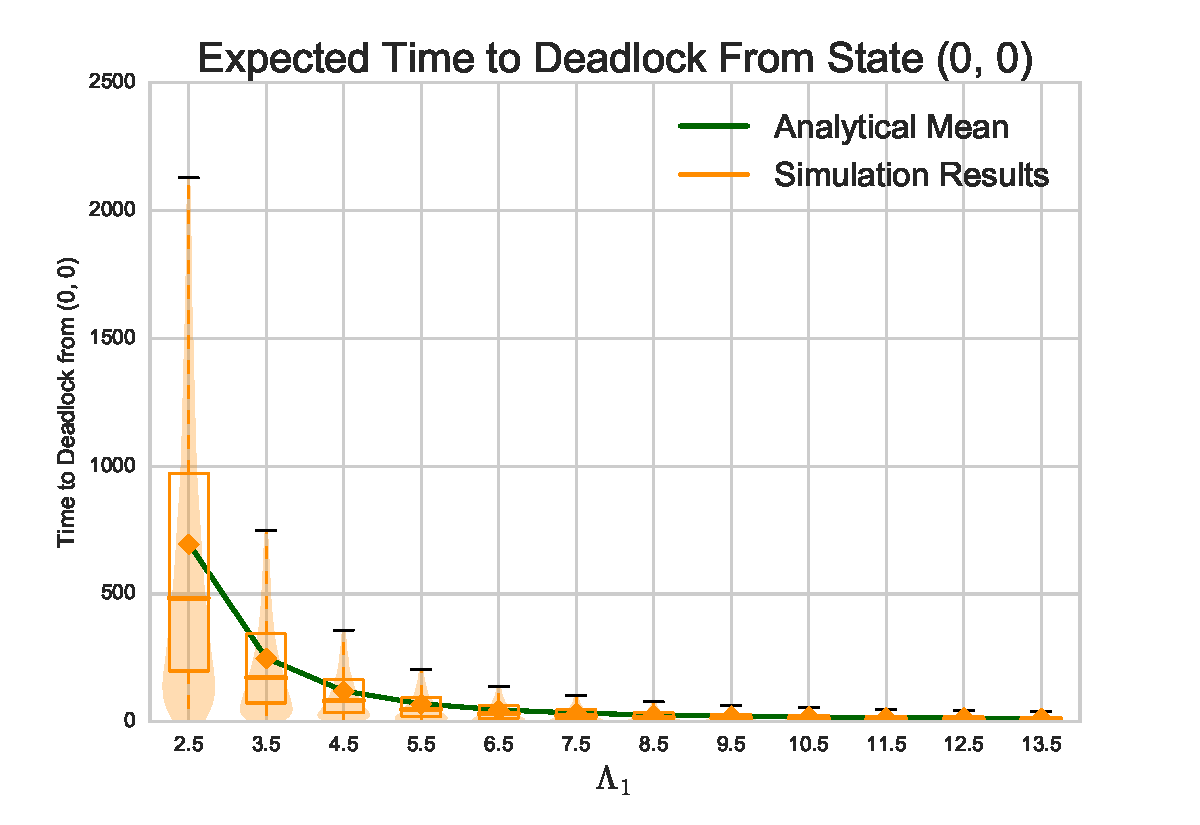
\includegraphics[width=\textwidth]{images/varyL1}
  \caption{Varying $\Lambda_1$}
  \label{fig:timestodeadlock2_L1}
\end{subfigure}
\begin{subfigure}[b]{0.38\textwidth}
  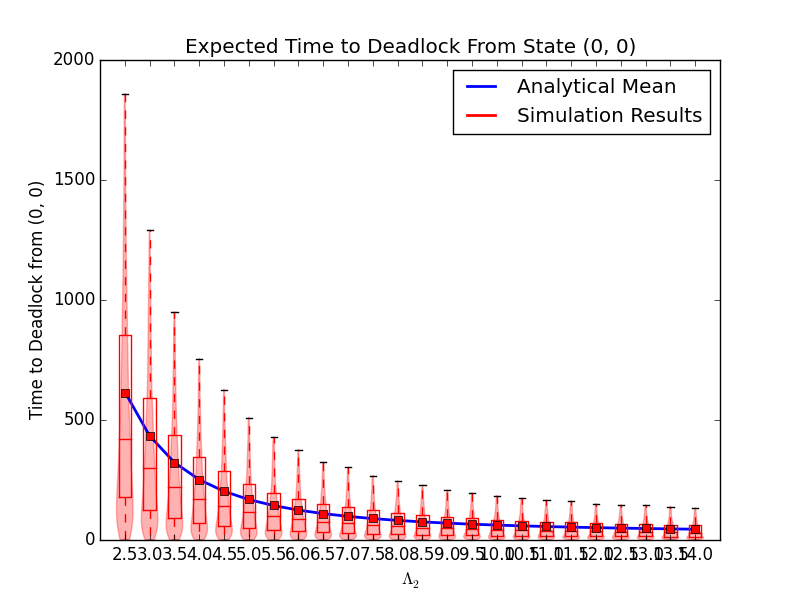
\includegraphics[width=\textwidth]{images/varyL2}
  \caption{Varying $\Lambda_2$}
  \label{fig:timestodeadlock2_L2}
\end{subfigure}
\begin{subfigure}[b]{0.38\textwidth}
  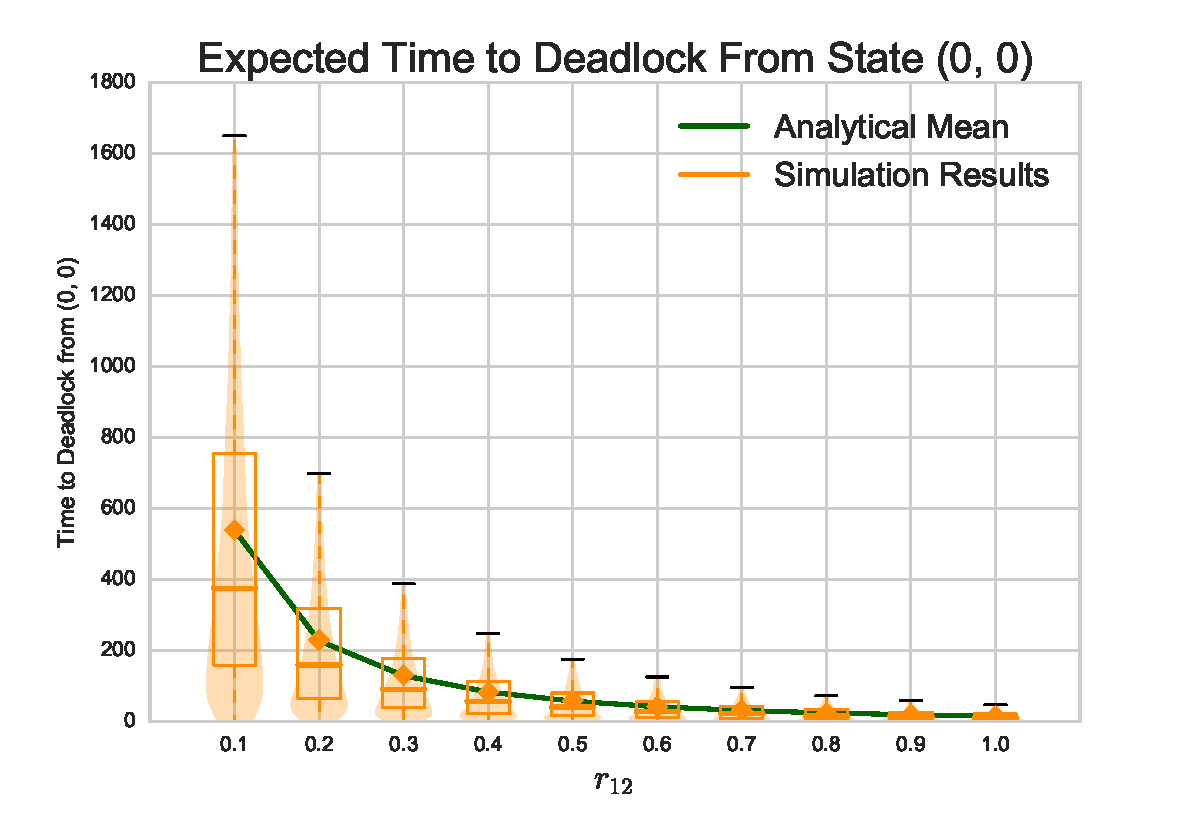
\includegraphics[width=\textwidth]{images/varyr12}
  \caption{Varying $r_{12}$}
  \label{fig:timestodeadlock2_r12}
\end{subfigure}
\begin{subfigure}[b]{0.38\textwidth}
  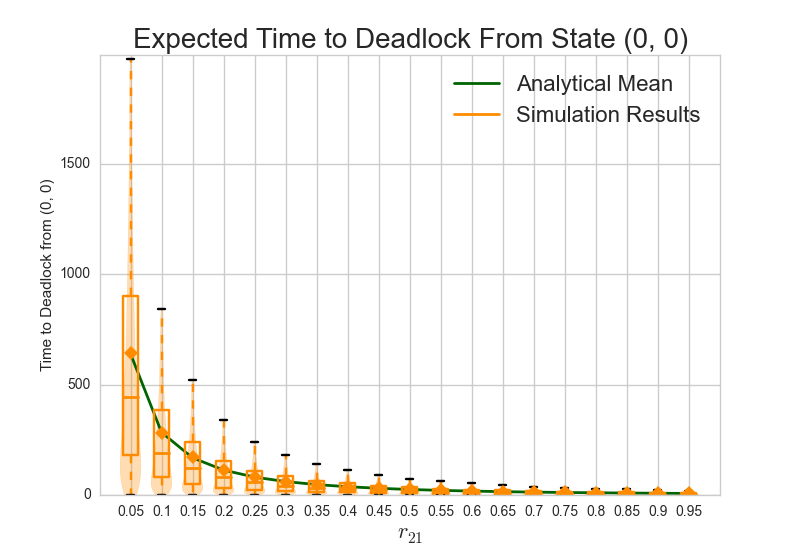
\includegraphics[width=\textwidth]{images/varyr21}
  \caption{Varying $r_{21}$}
  \label{fig:timestodeadlock2_r21}
\end{subfigure}
\begin{subfigure}[b]{0.38\textwidth}
  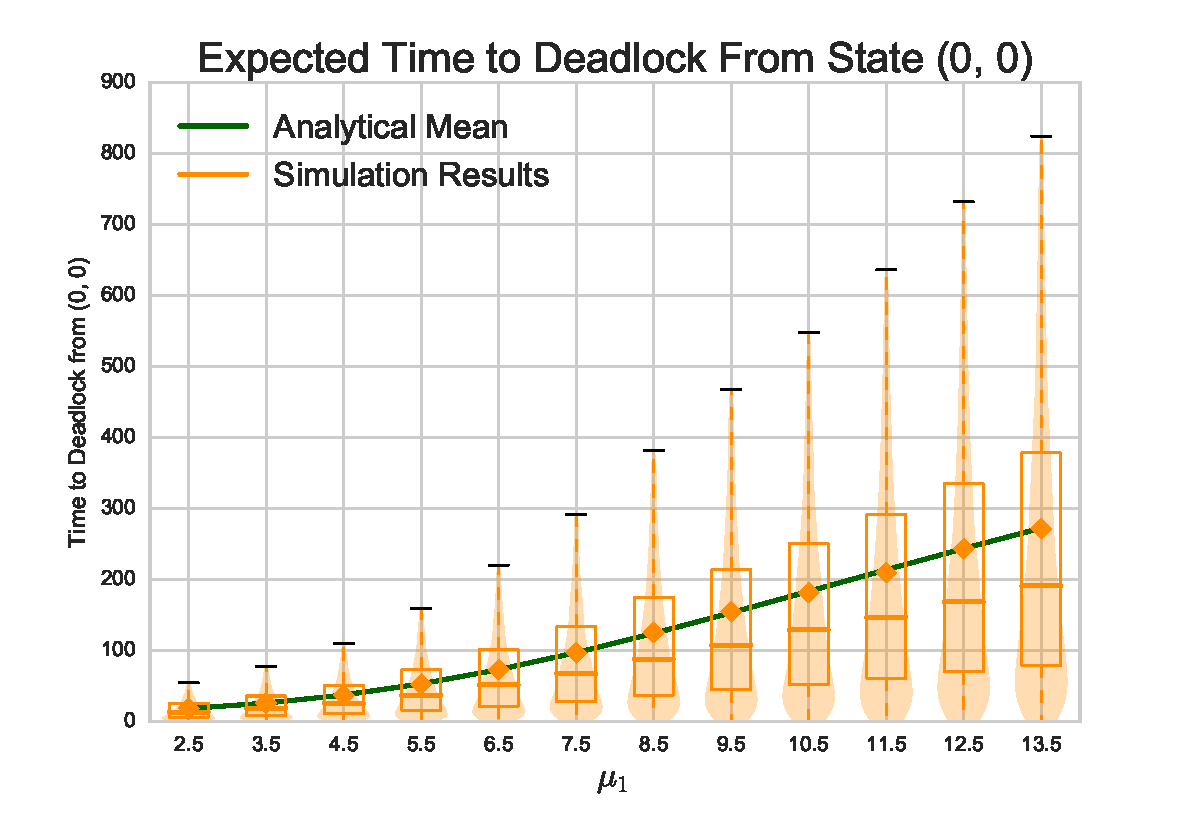
\includegraphics[width=\textwidth]{images/varymu1}
  \caption{Varying $\mu_1$}
  \label{fig:timestodeadlock2_mu1}
\end{subfigure}
\begin{subfigure}[b]{0.38\textwidth}
  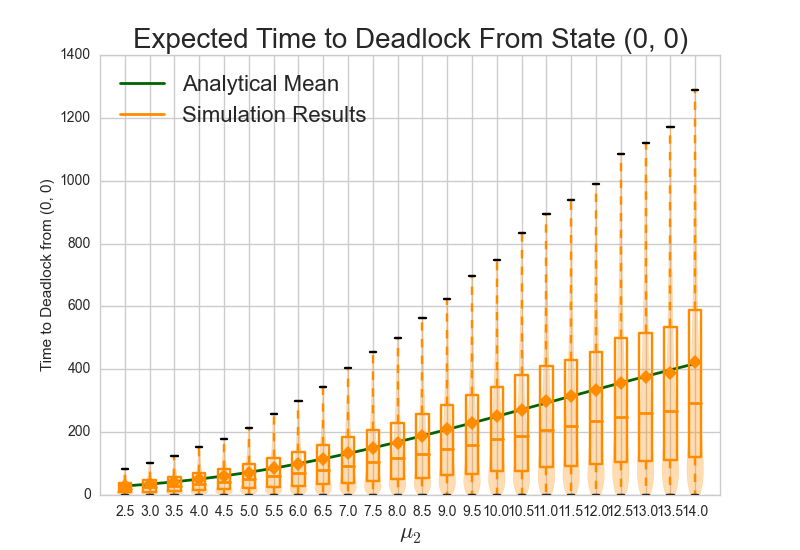
\includegraphics[width=\textwidth]{images/varymu2}
  \caption{Varying $\mu_2$}
  \label{fig:timestodeadlock2_mu2}
\end{subfigure}
\begin{subfigure}[b]{0.38\textwidth}
  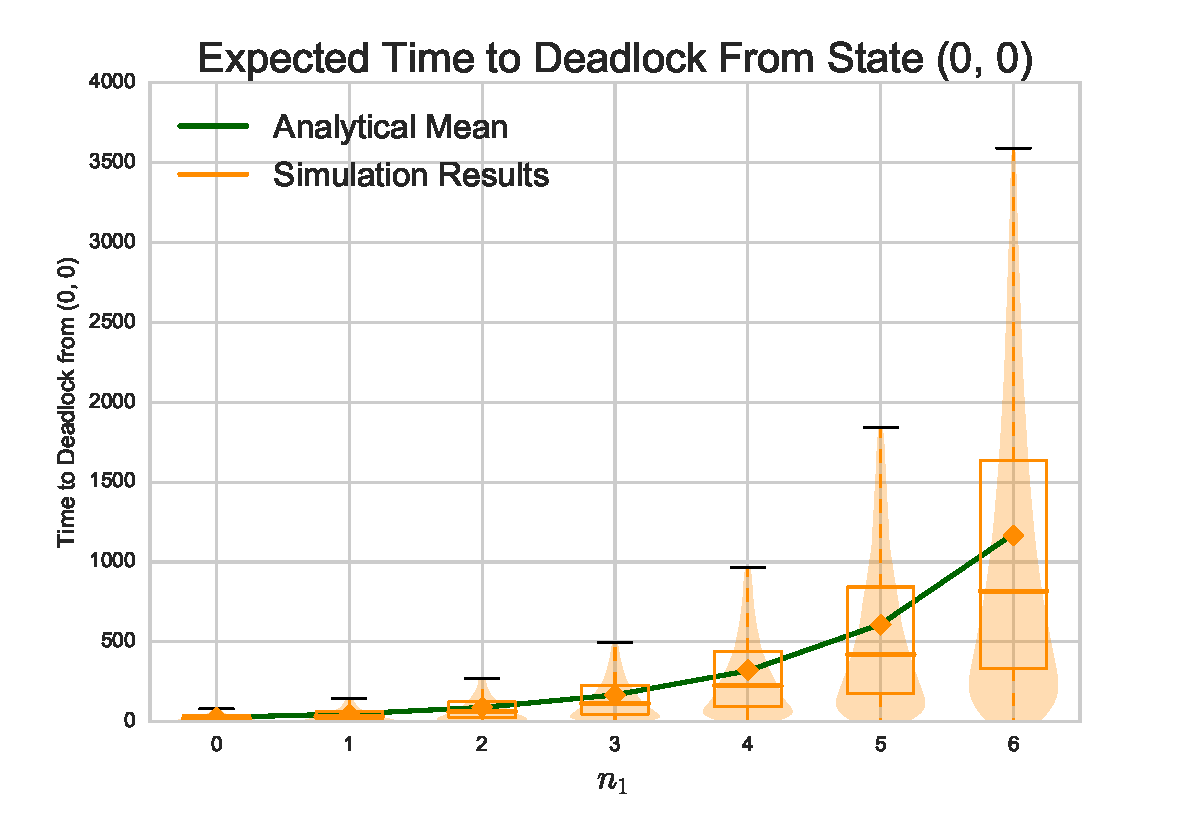
\includegraphics[width=\textwidth]{images/varyn1}
  \caption{Varying $n_1$}
  \label{fig:timestodeadlock2_n1}
\end{subfigure}
\begin{subfigure}[b]{0.38\textwidth}
  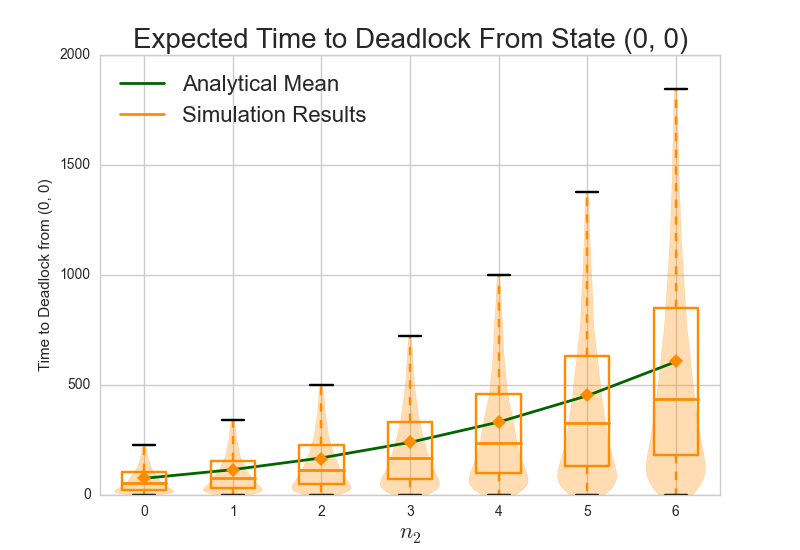
\includegraphics[width=\textwidth]{images/varyn2}
  \caption{Varying $n_2$}
  \label{fig:timestodeadlock2_n2}
\end{subfigure}
\end{center}
\caption{Time to deadlock in $\Omega_2$, analytical \& simulation results (10,000 iterations).}
\label{fig:timestodeadlock2}
\end{figure}
\end{center}










\subsection{Two Node Single-Server with Self-Loops}\label{sec:2nodeselfloops}

Consider the open two node single-server restricted queueing network shown in Figure~\ref{fig:queueingnetwork_2nodesfeedback}.
This shows two \(M/M/1/n_i\) queues with service rates $\mu_i$  and external arrival rates $\Lambda_i$.
All routing possibilities are possible, where the routing probability from node $i$ to node $j$ is denoted by $r_{ij}$.

Let this system be denoted by $\Omega$ with parameter set $(\Lambda_1$, $\Lambda_2$, $\mu_1$, $\mu_2$, $n_1$, $n_2$, $r_{11}$, $r_{12}$, $r_{21}$, $r_{22})$.

\begin{figure}[!htbp]
  \begin{center}
  \includestandalone[width=0.75\textwidth]{images/2nodefeedbackexample}
  \end{center}
  \caption{An open two node single-server restricted queueing network.}
  \label{fig:queueingnetwork_2nodesfeedback}
\end{figure}

State space:
    \[S = \{(i,j)\in\mathbb{N}^{(n_1+2\times n_2+2)} \nonscript\; | \nonscript\; 0 \leq i + j \leq n_1 + n_2 + 2
    \}\cup\{(-1), (-2), (-3)\}\]

    where \(i\) denotes the number of individuals:
        \begin{itemize}
            \item In service or waiting at the first node.
            \item Occupying a server but having finished service at the
                second node waiting to join the first.
        \end{itemize}
    where \(j\) denotes the number of individuals:
        \begin{itemize}
            \item In service or waiting at the second node.
            \item Occupying a server but having finished service at the
                first node waiting to join the second.
        \end{itemize}
    and the state $(-3)$ denotes the deadlocked state cause by both nodes; $(-1)$ denotes the deadlocked state caused by the first node only; and $(-2)$ denotes the deadlocked state caused by the second node only.

Define $\delta = (i_2, j_2) - (i_1, j_1)$ for all $(i_k, j_k) \in S$. The transitions are given by:

\begin{equation}
  q_{(i_1, j_1),(i_2, j_2)} = \left\{
  \begin{matrix*}[ r ]
    \left. \begin{matrix*}[ r ]
      \Lambda_1 & \text{if } i_1 < n_1 + 1 \\
      0 & \text{otherwise}
    \end{matrix*} \right\} & \text{if } \delta = (1, 0) \\
    \left. \begin{matrix*}[ r ]
      \Lambda_2 & \text{if } j_1 < n_2 + 1 \\
      0 & \text{otherwise}
    \end{matrix*} \right\} & \text{if } \delta = (0, 1) \\
    \left. \begin{matrix*}[ r ]
      (1 - r_{11} - r_{12})\mu_1 & \text{if } j_1 < n_2 + 2 \\
      0 & \text{otherwise}
    \end{matrix*} \right\} & \text{if } \delta = (-1, 0) \\
    \left. \begin{matrix*}[ r ]
      (1 - r_{21} - r_{22})\mu_2 & \text{if } i_1 < n_1 + 2 \\
      0 & \text{otherwise}
    \end{matrix*} \right\} & \text{if } \delta = (0, -1) \\
    \left. \begin{matrix*}[ r ]
      r_{12}\mu_1 & \text{if } j_1 < n_2 + 2 \text{ and } (i_1, j_1) \neq (n_1 + 2, n_2) \\
      0 & \text{otherwise}
    \end{matrix*} \right\} & \text{if } \delta = (-1, 1) \\
    \left. \begin{matrix*}[ r ]
      r_{21}\mu_2 & \text{if } i_1 < n_1 + 2 \text{ and } (i_1, j_1) \neq (n_1, n_2 + 2) \\
      0 & \text{otherwise}
    \end{matrix*} \right\} & \text{if } \delta = (1, -1) \\
    0 & \text{otherwise}
  \end{matrix*} \right.
\end{equation}

\begin{equation}\label{equ:todeadlock2}
  q_{(i_1, j_1), (-1)} = \left\{
  \begin{matrix*}[ r ]
    r_{11}\mu_1 & \text{if } i > n_1 \text{ and } j < n_2 + 2 \\
    0 & \text{otherwise}
  \end{matrix*}
  \right.
\end{equation}

\begin{equation}\label{equ:todeadlock3}
  q_{(i_1, j_1), (-2)} = \left\{
  \begin{matrix*}[ r ]
    r_{22}\mu_2 & \text{if } j > n_2 \text{ and } i < n_1 + 2 \\
    0 & \text{otherwise}
  \end{matrix*}
  \right.
\end{equation}

\begin{equation}
  q_{(i_1, j_1), (-3)} = \left\{
  \begin{matrix*}[ r ]
    r_{21}\mu_2 & \text{if } (i, j) = (n_1, n_2 + 2) \\
    r_{12}\mu_1 & \text{if } (i, j) = (n_1 + 2, n_2) \\
    0 & \text{otherwise}
  \end{matrix*}
  \right.
\end{equation}

\begin{align}
  q_{-1, s} = 0 \\
  q_{-2, s} = 0 \\
  q_{-3, s} = 0
\end{align}

Note that there are only two differences between this formulation and the formulation given in Subsection~\ref{sec:2nodewithoutselfloops}: the rates at which customers leave nodes 1 and 2 are now $(1-r_{11}-r_{12})\mu_1$ and $(1-r_{21}-r_{22})\mu_2$; and there are now two more ways to reach deadlock, Equation~\ref{equ:todeadlock2} and Equation~\ref{equ:todeadlock3}.

For $n_1 = 1$ and $n_2 = 2$, the resulting Markov chain is shown in Figure~\ref{fig:2nodeMCfeedback}.

\begin{figure}[!htbp]
    \begin{center}
    \includestandalone[width=0.75\textwidth]{images/markov_chain_feedback}
    \end{center}
    \caption{Diagrammatic representation of the Markov chain for $\Omega$ with $n_1=1$ and $n_2=2$.}
    \label{fig:2nodeMCfeedback}
\end{figure}

Figure~\ref{fig:timestodeadlockfeedback} shows the effect of varying the parameters of the above Markov model.
Base parameters of $\Lambda_1 = 4$, $\Lambda_2 = 5$, $n_1 = 3$, $n_2 = 2$, $\mu_1 = 10$, $\mu_2 = 8$, $r_{11} = 0.1$, $r_{12} = 0.25$, $r_{21} = 0.15$ and $r_{22} = 0.1$ are used.


\begin{figure}[!htbp]
\begin{center}
\begin{subfigure}[b]{0.35\textwidth}
  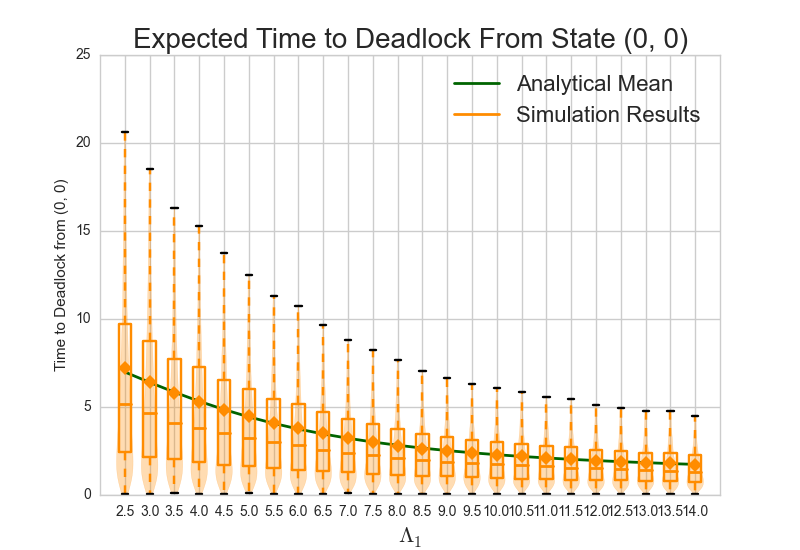
\includegraphics[width=\textwidth]{images/vary_L1fb}
  \caption{Varying $\Lambda_1$}
  \label{fig:timestodeadlockfb_L1}
\end{subfigure}
\begin{subfigure}[b]{0.35\textwidth}
  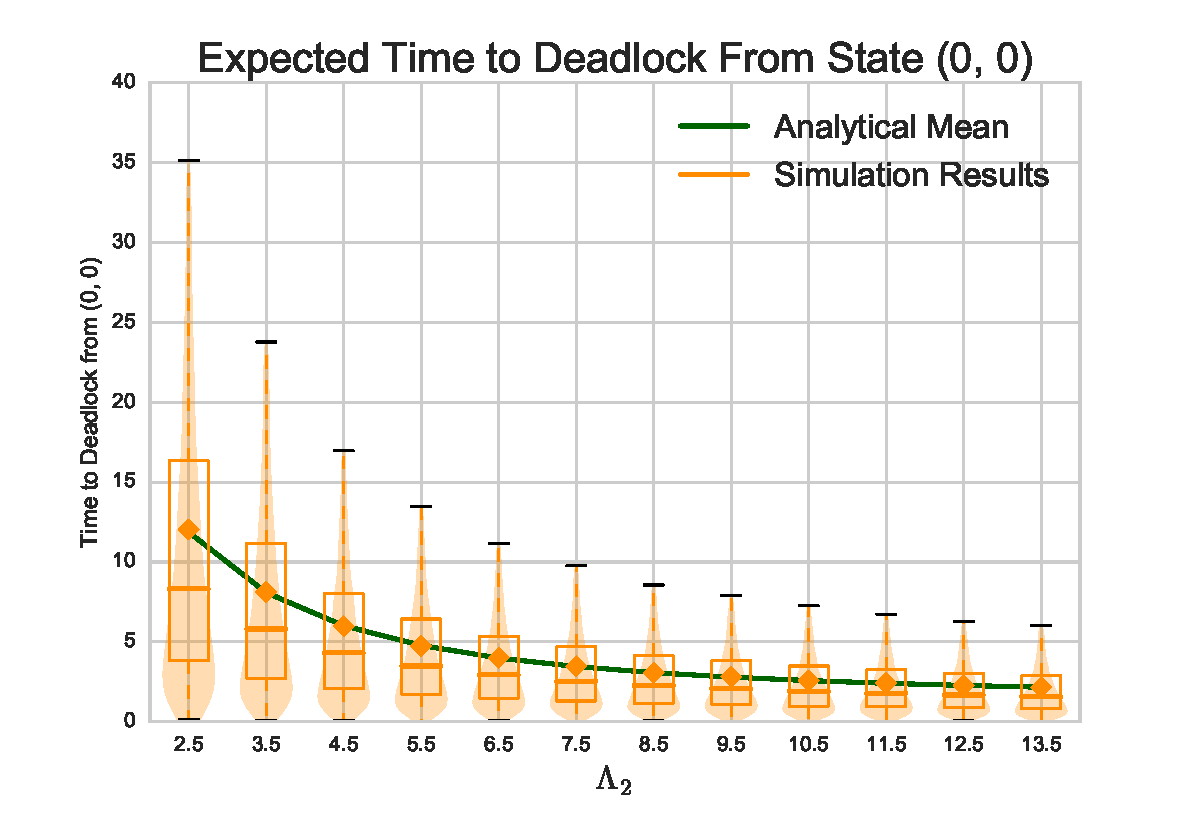
\includegraphics[width=\textwidth]{images/vary_L2fb}
  \caption{Varying $\Lambda_2$}
  \label{fig:timestodeadlockfb_L2}
\end{subfigure}\\
\begin{subfigure}[b]{0.35\textwidth}
  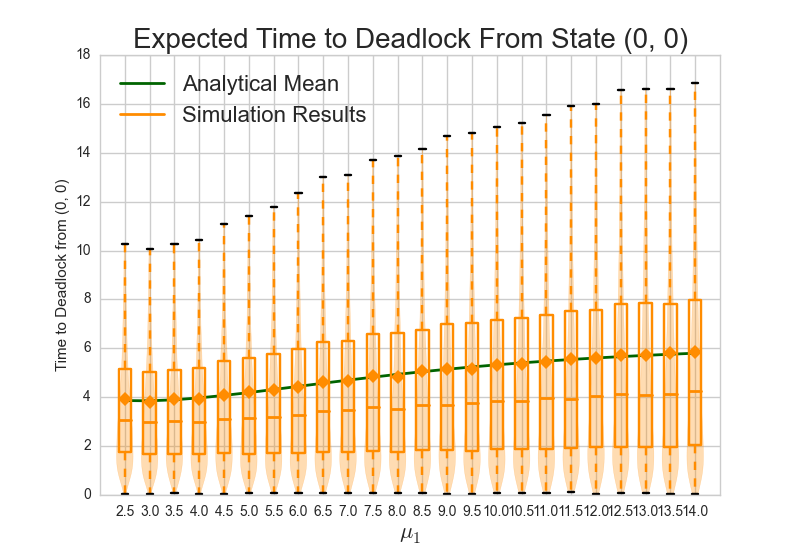
\includegraphics[width=\textwidth]{images/vary_mu1fb}
  \caption{Varying $\mu_1$}
  \label{fig:timestodeadlockfb_mu1}
\end{subfigure}
\begin{subfigure}[b]{0.35\textwidth}
  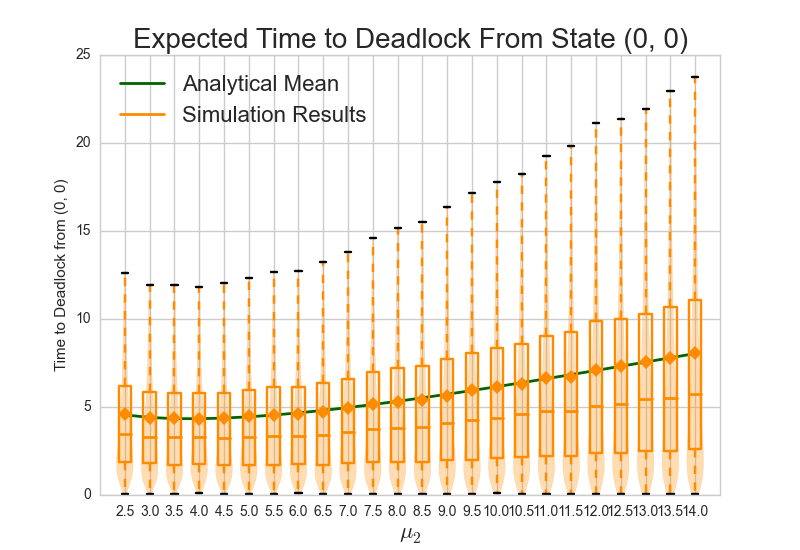
\includegraphics[width=\textwidth]{images/vary_mu2fb}
  \caption{Varying $\mu_2$}
  \label{fig:timestodeadlockfb_mu2}
\end{subfigure}\\
\begin{subfigure}[b]{0.35\textwidth}
  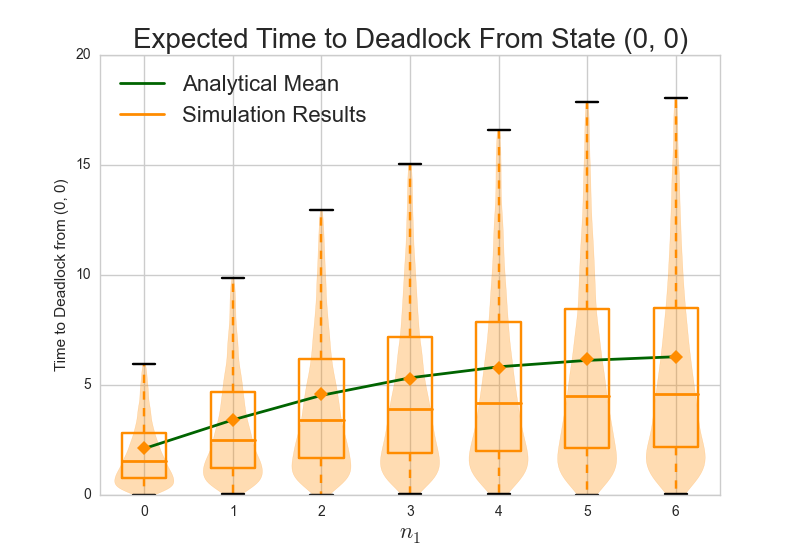
\includegraphics[width=\textwidth]{images/vary_n1fb}
  \caption{Varying $n_1$}
  \label{fig:timestodeadlockfb_n1}
\end{subfigure}
\begin{subfigure}[b]{0.35\textwidth}
  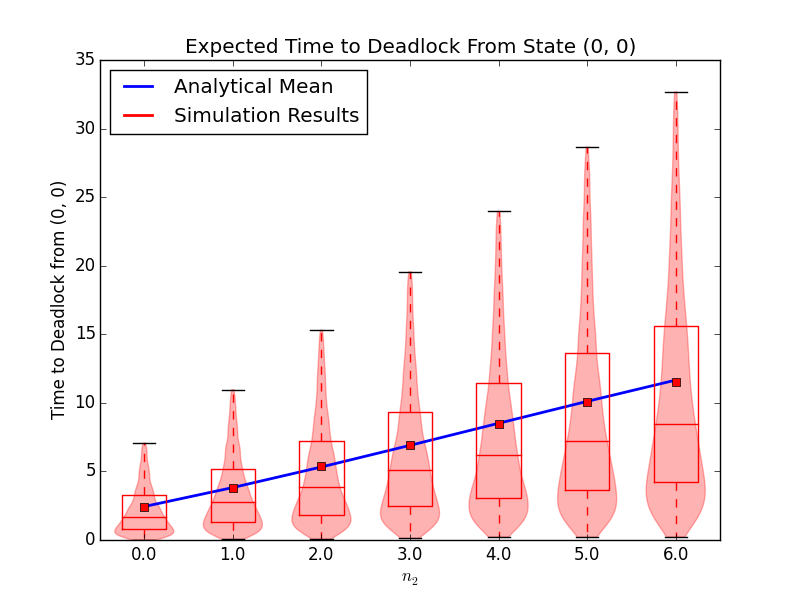
\includegraphics[width=\textwidth]{images/vary_n2fb}
  \caption{Varying $n_2$}
  \label{fig:timestodeadlockfb_n2}
\end{subfigure}
\end{center}
\caption{Time to deadlock in $\Omega$, analytical \& simulation results (10,000 iterations).}
% You cannot see the violins in these plots. Not sure how to fix.
\label{fig:timestodeadlockfeedback}
\end{figure}

\subsection{One Node Multi-Server}\label{sec:1nodeMS}

Consider the open one node multi-server restricted queueing network shown in Figure~\ref{fig:queueingnetwork_1nodemulti}.
This is an $\Omega_1$ system with $c$ parallel servers.

\begin{figure}[!htbp]
  \begin{center}
  \includestandalone[width=0.75\textwidth]{images/1nodemultiserver}
  \end{center}
  \caption{An open one node multi-server restricted queueing network.}
  \label{fig:queueingnetwork_1nodemulti}
\end{figure}

State space:
        \[S = \{i\in\mathbb{N} \nonscript\; | \nonscript\; 0 \leq i \leq n + 2c\}\]
where \(i\) denotes the number of individuals in the system plus the number of individuals blocked who are blocked.
For example, $i=n+c+2$ denotes a full system, $n+c$ individuals in the node, and 2 of those individuals are also blocked.
The state $i=n+2c$ denotes the deadlocked state.

Define $\delta = i_2 - i_1$ for all $i_k \in S$. The transitions are given by:

\begin{equation}
  q_{i_1, i_2} = \left\{
  \begin{matrix*}[ r ]
    \left. \begin{matrix*}[ r ]
      \Lambda & \text{if } \delta = 1 \\
      (1-r_{11})\mu\text{min}(i, c) & \text{if } \delta = -1 \\
      0 & \text{otherwise}
    \end{matrix*} \right\} & \text{if } i_1 < n + c \\
  \end{matrix*} \right.
\end{equation}

\begin{equation}
  q_{i_1, i_2} = \left\{
  \begin{matrix*}[ r ]
    \left. \begin{matrix*}[ r ]
      (c-b)r_{11}\mu & \text{if } \delta = 1 \\
      (1-r_{11})(b-k)\mu & \text{if } \delta = -b-1\\
      0 & \text{otherwise}
    \end{matrix*} \right\} & \text{if } i_1 = n + c + b \\
  \end{matrix*} \right.
  \quad \forall \quad 0 \leq b \leq c
\end{equation}

where $b$ denotes the number of blocked customers.
The Markov chain is shown in Figure~\ref{fig:1nodeMCms}.

\begin{figure}[!htbp]
    \begin{center}
    \includestandalone[width=0.75\textwidth]{images/MC1nodemultiserv}
    \end{center}
    \caption{Diagrammatic representation of the Markov chain for a multi-server $\Omega_1$ system.}
    \label{fig:1nodeMCms}
\end{figure}

Increasing the amount of servers has a similar effect to increasing the queueing capacity, there are now more transient states to go through before reaching the deadlocked state.
Varying the amount of servers has a greater effect on the time to deadlock however, as any states in which customers are blocked ($i \in [n+c+1, i=n+2c]$) can jump back to state $i=n+c-1$ simply with a service and an exit.
Increasing the amount of servers also increases the rate at which $i$ are reduced for most states, but not the rates at which $i$ is increased.

Figure~\ref{fig:timestodeadlock1nodemultiserver} shows the effect of varying the parameters of the above Markov model.
Base parameters of $\Lambda = 6$, $n = 3$, $\mu = 2$, $r_{11} = 0.5$ and $c = 2$ were used.

\begin{figure}[!htbp]
  \begin{center}
  \begin{subfigure}[b]{0.35\textwidth}
    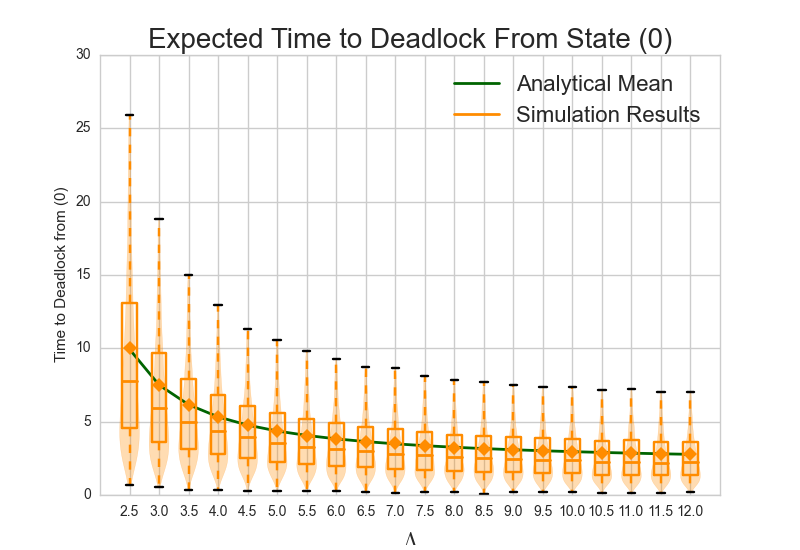
\includegraphics[width=\textwidth]{images/varyL_1Nms}
    \caption{Varying $\Lambda$}
    \label{fig:1Nms_L}
  \end{subfigure}
  \begin{subfigure}[b]{0.35\textwidth}
    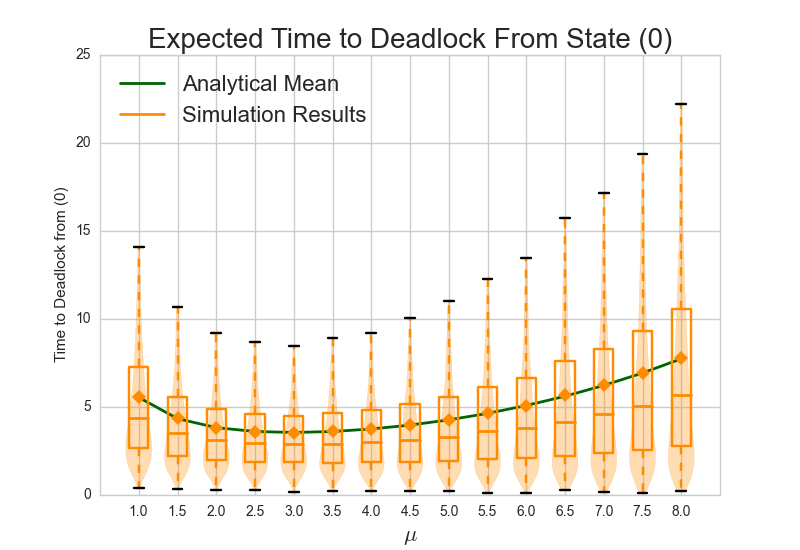
\includegraphics[width=\textwidth]{images/varymu_1Nms}
    \caption{Varying $\mu$}
    \label{fig:1Nms_mu}
  \end{subfigure}\\
  \begin{subfigure}[b]{0.35\textwidth}
    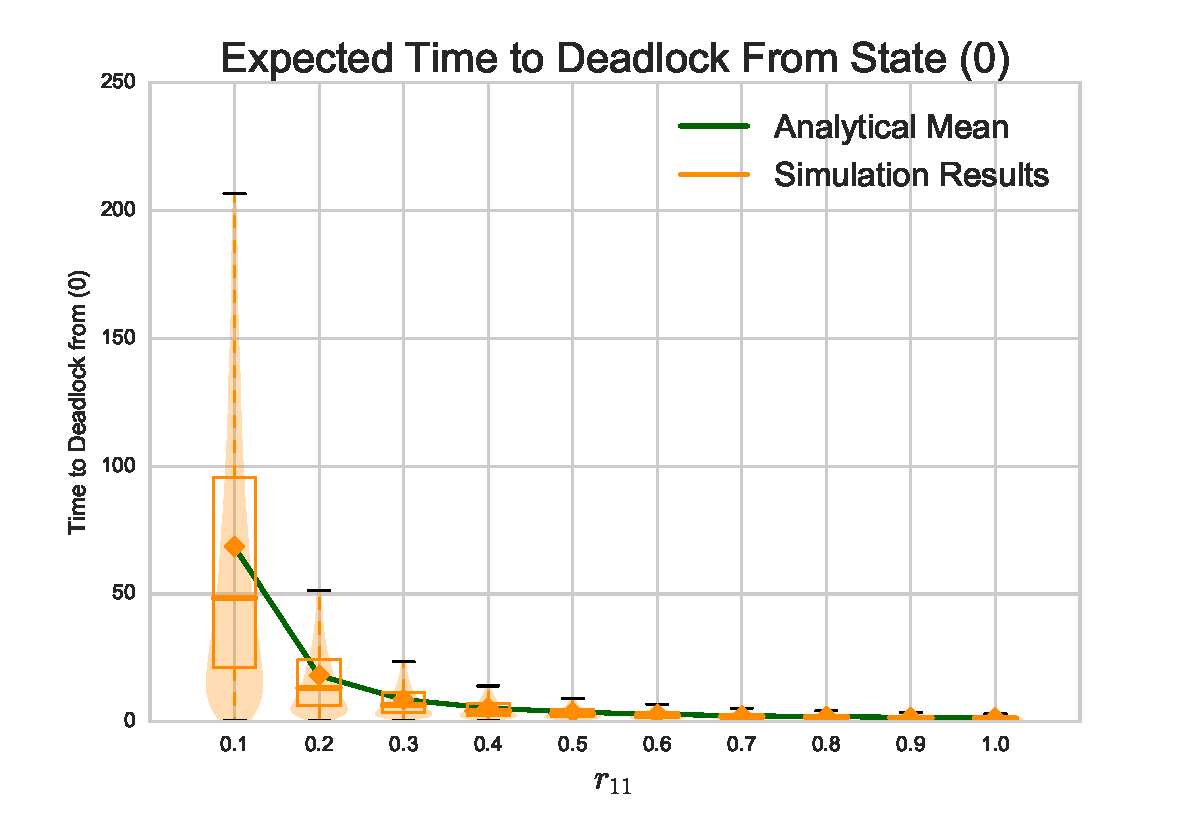
\includegraphics[width=\textwidth]{images/varyr11_1Nms}
    \caption{Varying $r_{11}$}
    \label{fig:1Nms_r11}
  \end{subfigure}
  \begin{subfigure}[b]{0.35\textwidth}
    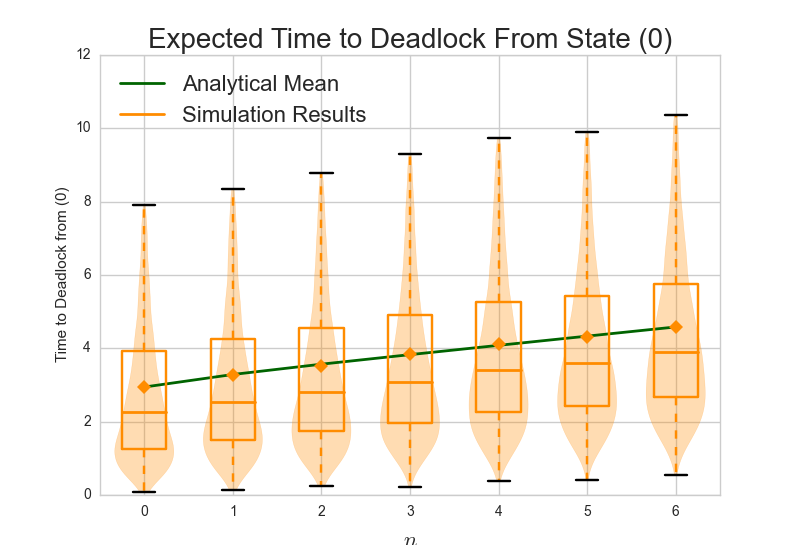
\includegraphics[width=\textwidth]{images/varyn_1Nms}
    \caption{Varying $n$}
    \label{fig:1Nms_n}
  \end{subfigure}\\
  \begin{subfigure}[b]{0.35\textwidth}
    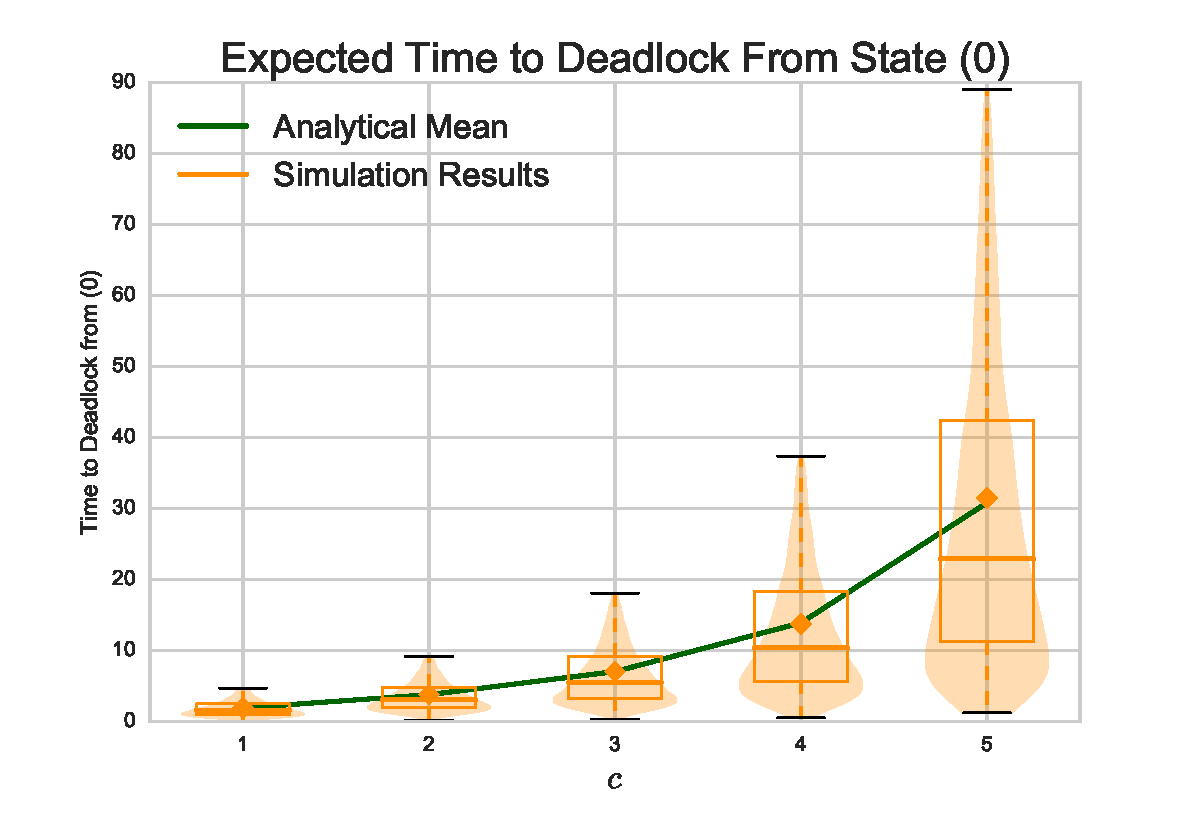
\includegraphics[width=\textwidth]{images/varyc_1Nms}
    \caption{Varying $c$}
    \label{fig:1Nms_c}
  \end{subfigure}
  \end{center}
  \caption{Time to deadlock in multi-server $\Omega_1$, analytical \& simulation results (10,000 iterations).}
  \label{fig:timestodeadlock1nodemultiserver}
\end{figure}











\subsection{Two Node Multi-Server without Self-Loops}\label{sec:2nodeMS}

Consider the open two node mutli server restricted queueing network shown in Figure~\ref{fig:queueingnetwork_2nodemulti}.
This is an $\Omega_2$ system with $c_i$ parallel servers at node $i$.

\begin{figure}[!htbp]
  \begin{center}
  \includestandalone[width=0.75\textwidth]{images/2nodemultiserver}
  \end{center}
  \caption{An open two node mutli server restricted queueing network.}
  \label{fig:queueingnetwork_2nodemulti}
\end{figure}

State space:
        \[S = \{(i,j)\in\mathbb{N}^{(n_1+c_1+c_2)\times (n_2+c_2+c_1)} \nonscript\; | \nonscript\; i \leq n_1+c_1+j, \nonscript\; j \leq n_2+c_2+i\}\]
where $i$ denotes the number of individuals at Node 1 plus the number of individuals blocked waiting to enter Node 1, and $j$ denotes the number of individuals at Node 2 plus the number of individuals blocked waiting to enter Node 2.
For example, $(i, j) = (n_1+c_1+2, n_2+c_2+1)$ denotes a full system, $n_1+c_1$ individuals at Node 1, two of whom are blocked waiting to enter Node 2; $n_2+c_2$ individuals at Node 2, one of whom is blocked waiting to enter Node 1.
The state $(i, j) = (n_1+c_1+c_2, n_2+c_2+c_1)$ denotes the deadlocked state.

The Markov chain is shown in Figure~\ref{fig:2nodeMCms}.

\begin{figure}[!htbp]
    \includestandalone[width=\textwidth]{images/MC2nodemultiserv}
    \caption{Diagrammatic representation of the Markov chain for a multi-server $\Omega_2$ system with $n_1=1$, $n_2=c_1=c_2=2$. The deadlocked state is $(5,6)$.}
    \label{fig:2nodeMCms}
\end{figure}

Define $\delta = (i_2, j_2) - (i_1, j_1)$, $b_1 = \max(0, i_1-n_1-c_1)$, $b_2 = \max(0, i_2-n_2-c_2)$, $s_1 = \min(i_1, c_1)-b_2$ and $s_2 = \min(i_2, c_2)-b_1$ for all $(i_k, j_k) \in S$.
Then the transitions $q_{(i_1, j_1),(i_2, j_2)}$ are given by Table~\ref{tab:transitionsmultierv}.


\begin{table}
\begin{center}
\resizebox{\textwidth}{!}{
\begin{tabular}{ l | l | l | l |}
  & $j_1 < n_2 + c_2$ & $j_1 = n_2 + c_2$ & $ j_1 > n_2 + c_2$ \\ \hline
  $i_1 < n_1 + c_1$ & \begin{tabular}{ l } $\Lambda_1$ if $\delta = (1, 0)$ \\ $\Lambda_2$ if $\delta = (0, 1)$ \\ $r_{12}s_1\mu_1$ if $\delta = (-1, 1)$ \\ $r_{21}s_2\mu_2$ if $\delta = (1, -1)$ \\ $(1-r_{12})s_1\mu_1$ if $\delta = (-1, 0)$ \\ $(1-r_{21})s_2\mu_2$ if $\delta = (0, -1)$ \end{tabular} & \begin{tabular}{ l } $\Lambda_1$ if $\delta = (1, 0)$ \\ $r_{12}s_1\mu_1$ if $\delta = (0, 1)$ \\ $r_{21}s_2\mu_2$ if $\delta = (1, -1)$ \\ $(1-r_{12})s_1\mu_1$ if $\delta = (-1, 0)$ \\ $(1-r_{21})s_2\mu_2$ if $\delta = (0, -1)$ \end{tabular} & \begin{tabular}{ l } $\Lambda_1$ if $\delta = (1, 0)$ \\ $r_{12}s_1\mu_1$ if $\delta = (0, 1)$ \\ $r_{21}s_2\mu_2$ if $\delta = (0, -1)$ \\ $(1-r_{12})s_1\mu_1$ if $\delta = (-1, 0)$ \\ $(1-r_{21})s_2\mu_2$ if $\delta = (-1, -1)$ \end{tabular} \\ \hline
  $i_1 = n_1 + c_1$ & \begin{tabular}{ l } $\Lambda_2$ if $\delta = (0, 1)$ \\ $r_{12}s_1\mu_1$ if $\delta = (-1, 1)$ \\ $r_{21}s_2\mu_2$ if $\delta = (1, 0)$ \\ $(1-r_{12})s_1\mu_1$ if $\delta = (-1, 0)$ \\ $(1-r_{21})s_2\mu_2$ if $\delta = (0, -1)$ \end{tabular} & \begin{tabular}{ l } $r_{12}s_1\mu_1$ if $\delta = (0, 1)$ \\ $r_{21}s_2\mu_2$ if $\delta = (1, 0)$ \\ $(1-r_{12})s_1\mu_1$ if $\delta = (-1, 0)$ \\ $(1-r_{21})s_2\mu_2$ if $\delta = (0, -1)$ \end{tabular} & \begin{tabular}{ l } $r_{12}s_1\mu_1$ if $\delta = (0, 1)$ \\ $r_{21}s_2\mu_2$ if $\delta = (1, 0)$ \\ $(1-r_{12})s_1\mu_1$ if $\delta = (-1, 0)$ \\ $(1-r_{21})s_2\mu_2$ if $\delta = (-1, -1)$ \end{tabular} \\ \hline
  $i_1 > n_1 + c_1$ & \begin{tabular}{ l } $\Lambda_2$ if $\delta = (0, 1)$ \\ $r_{12}s_1\mu_1$ if $\delta = (-1, 0)$ \\ $r_{21}s_2\mu_2$ if $\delta = (1, 0)$ \\ $(1-r_{12})s_1\mu_1$ if $\delta = (-1, -1)$ \\ $(1-r_{21})s_2\mu_2$ if $\delta = (0, -1)$ \end{tabular} & \begin{tabular}{ l } $r_{12}s_1\mu_1$ if $\delta = (0, 1)$ \\ $r_{21}s_2\mu_2$ if $\delta = (1, 0)$ \\ $(1-r_{12})s_1\mu_1$ if $\delta = (-1, -1)$ \\ $(1-r_{21})s_2\mu_2$ if $\delta = (0, -1)$ \end{tabular} & \begin{tabular}{ l } $r_{12}s_1\mu_1$ if $\delta = (0, 1)$ \\ $r_{21}s_2\mu_2$ if $\delta = (1, 0)$ \\ $(1-r_{12})s_1\mu_1$ if $\delta = (-\min(b_1+1,b_2+1), -\min(b_1,b_2+1))$ \\ $(1-r_{21})s_2\mu_2$ if $\delta = (-\min(b_1+1,b_2), -\min(b_1+1,b_2+1))$ \end{tabular} \\ \hline
\end{tabular}
}
\caption{Table of transitions $q_{(i_1, j_1),(i_2, j_2)}$ for a multi-server two node network.}
\label{tab:transitionsmultierv}
\end{center}
\end{table}


The values $b_1$ and $b_2$ correspond to the number of people blocked to Node 1 and Node 2 respectively.
The values $s_1$ and $s_2$ correspond to the amount of people currently in service at Node 1 and Node 2 respectively.

Figure~\ref{fig:timestodeadlock2nodemultiserver} shows the effect of varying the parameters of the above Markov model.
Base parameters of $\Lambda_1 = 9$, $\Lambda_2 = 7.5$, $n_1 = 2$, $n_2 = 1$, $\mu_1 = 5.5$, $\mu_2 = 6.5$, $r_{12} = 0.7$, $r_{21} = 0.6$, $c_1 = 2$ and $c_2 = 2$ were used.

\begin{figure}[!htbp]
  \begin{subfigure}[b]{0.333\textwidth}
    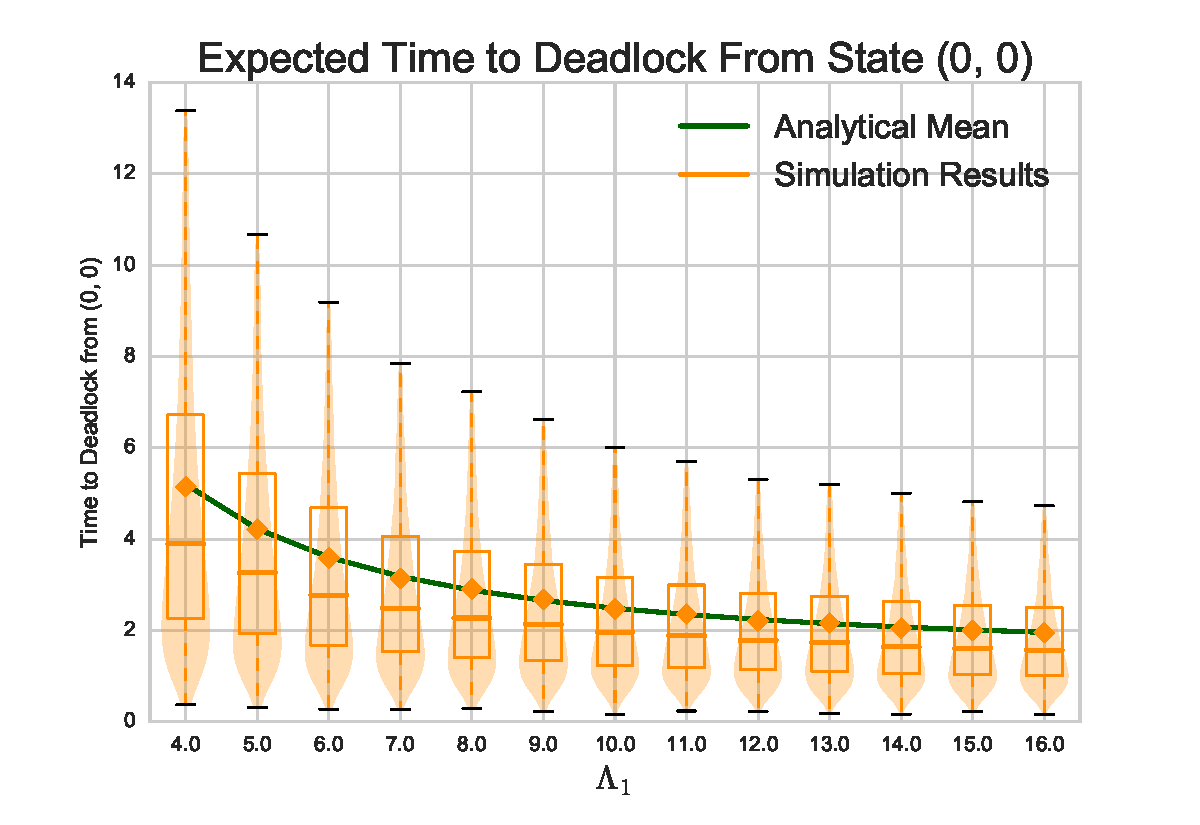
\includegraphics[width=\textwidth]{images/varyL1_2Nms}
    \caption{Varying $\Lambda_1$}
    \label{fig:2Nms_L1}
  \end{subfigure}
  \begin{subfigure}[b]{0.333\textwidth}
    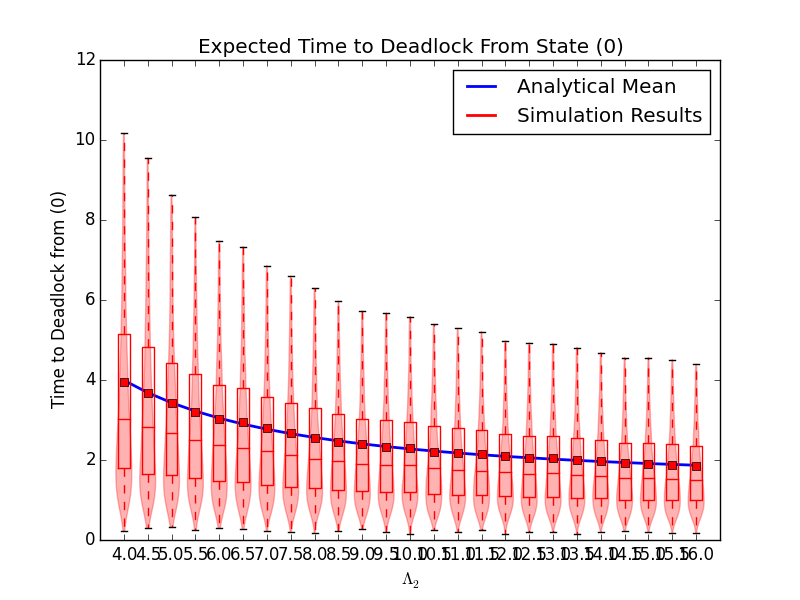
\includegraphics[width=\textwidth]{images/varyL2_2Nms}
    \caption{Varying $\Lambda_2$}
    \label{fig:2Nms_L2}
  \end{subfigure}
  \begin{subfigure}[b]{0.333\textwidth}
    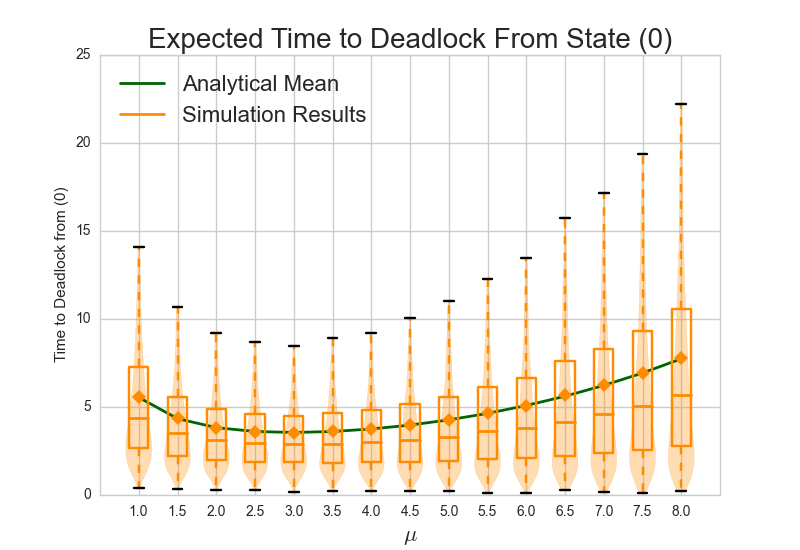
\includegraphics[width=\textwidth]{images/varymu_1Nms}
    \caption{Varying $\mu_1$}
    \label{fig:2Nms_mu1}
  \end{subfigure}
  \begin{subfigure}[b]{0.333\textwidth}
    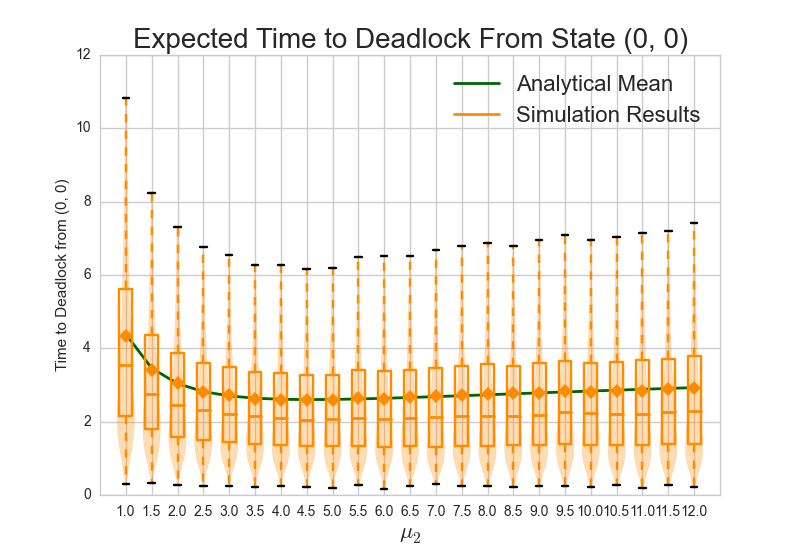
\includegraphics[width=\textwidth]{images/varymu2_2Nms}
    \caption{Varying $\mu_2$}
    \label{fig:2Nms_mu2}
  \end{subfigure}
  \begin{subfigure}[b]{0.333\textwidth}
    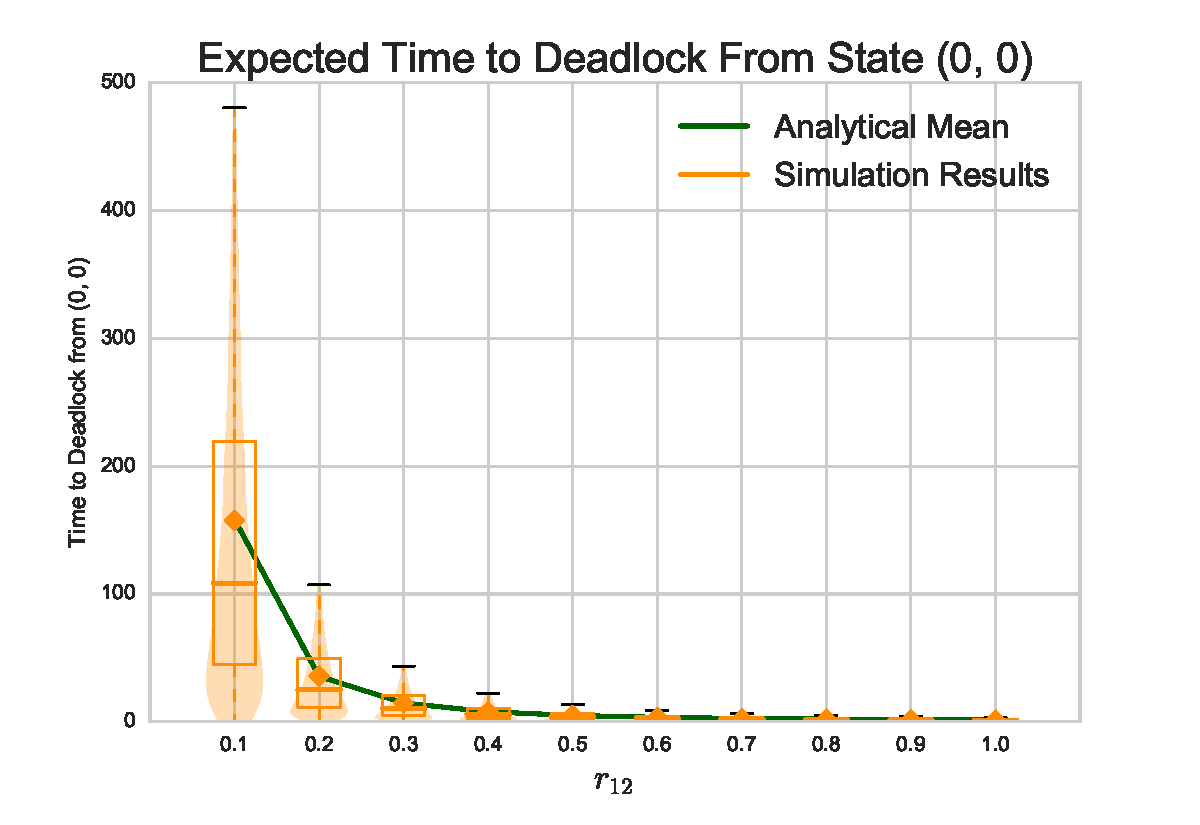
\includegraphics[width=\textwidth]{images/varyr12_2Nms}
    \caption{Varying $r_{12}$}
    \label{fig:2Nms_r12}
  \end{subfigure}
  \begin{subfigure}[b]{0.333\textwidth}
    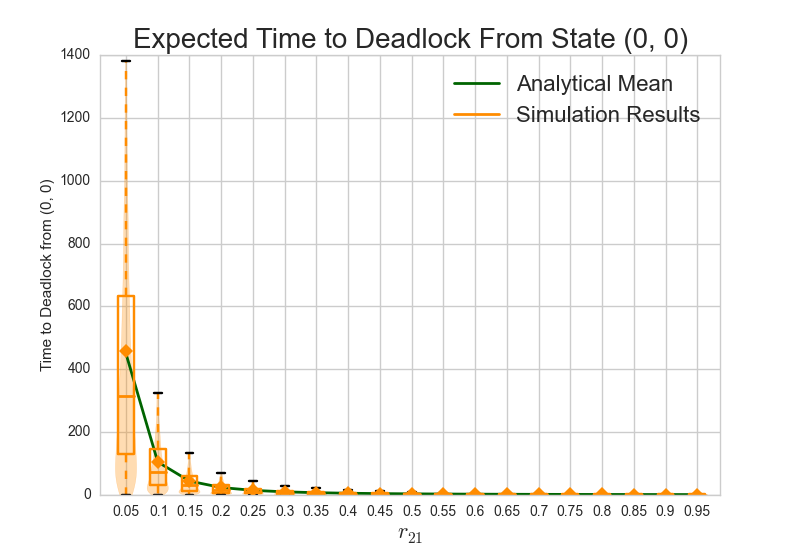
\includegraphics[width=\textwidth]{images/varyr21_2Nms}
    \caption{Varying $r_{21}$}
    \label{fig:2Nms_r21}
  \end{subfigure}
  \begin{center}
  \begin{subfigure}[b]{0.34\textwidth}
    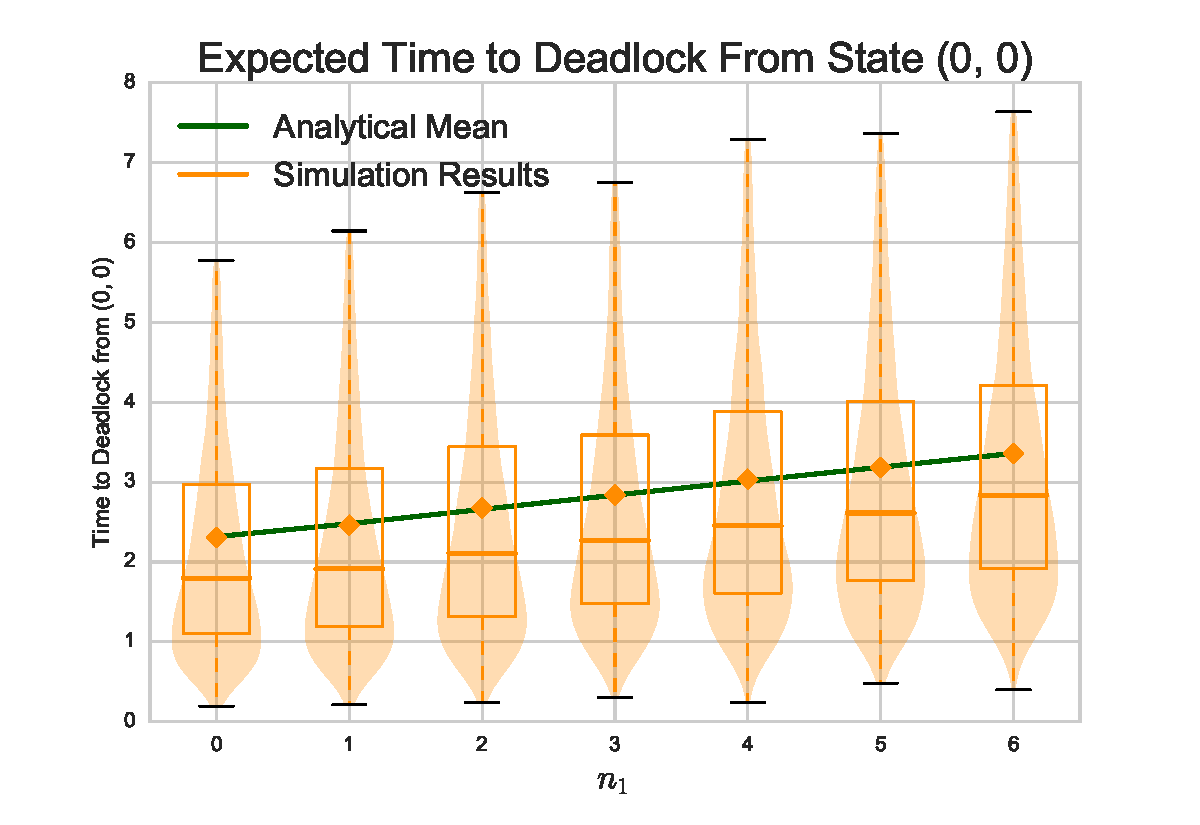
\includegraphics[width=\textwidth]{images/varyn1_2Nms}
    \caption{Varying $n_1$}
    \label{fig:2Nms_n1}
  \end{subfigure}
  \begin{subfigure}[b]{0.34\textwidth}
    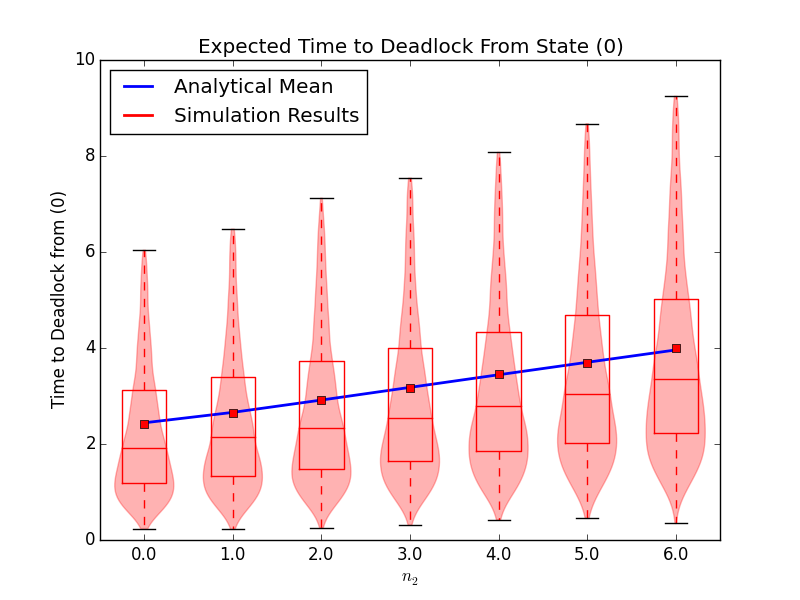
\includegraphics[width=\textwidth]{images/varyn2_2Nms}
    \caption{Varying $n_2$}
    \label{fig:2Nms_n2}
  \end{subfigure}
  \begin{subfigure}[b]{0.34\textwidth}
    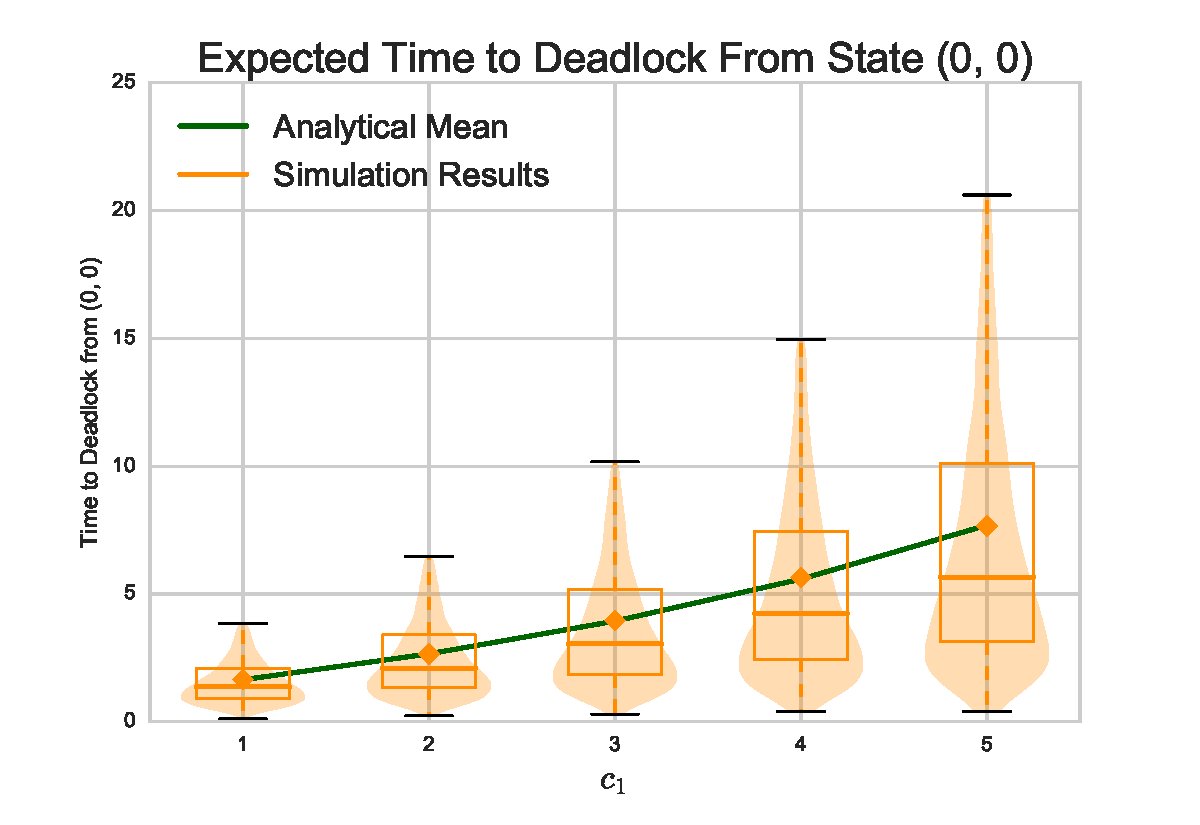
\includegraphics[width=\textwidth]{images/varyc1_2Nms}
    \caption{Varying $c_1$}
    \label{fig:2Nms_c1}
  \end{subfigure}
  \begin{subfigure}[b]{0.34\textwidth}
    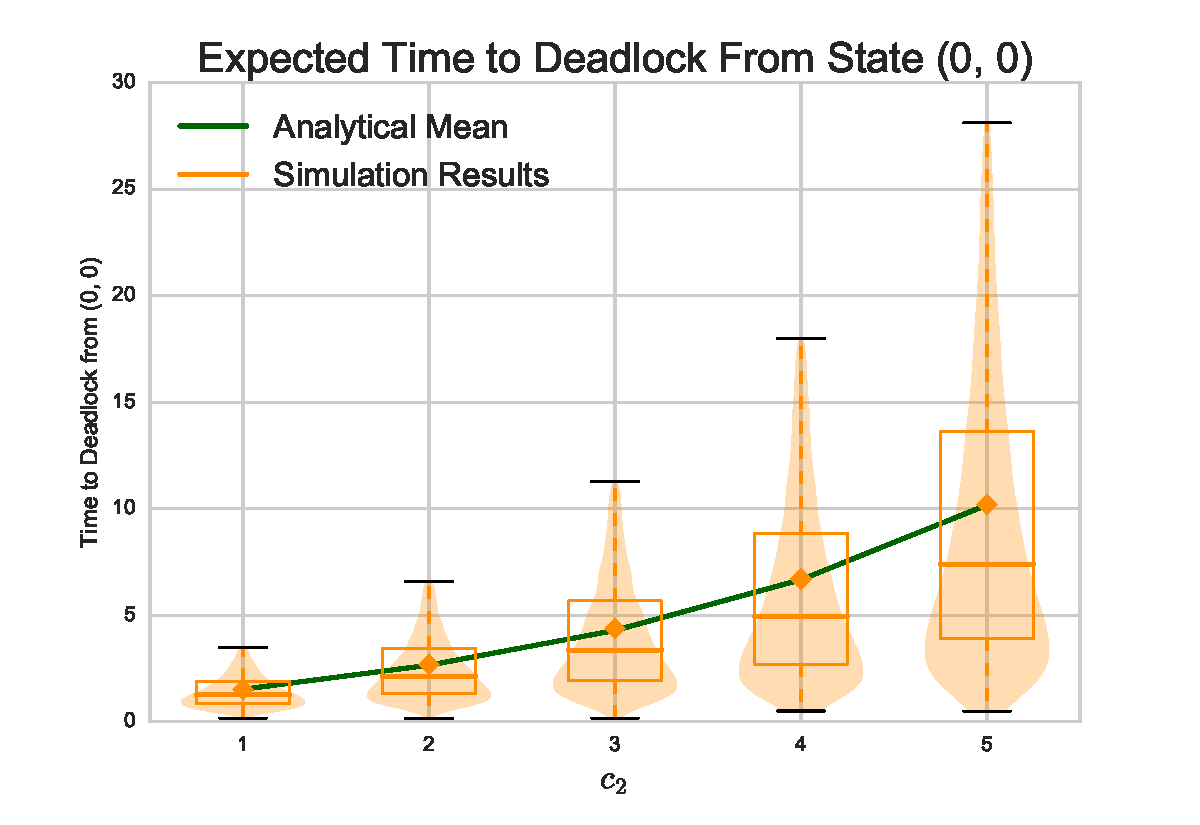
\includegraphics[width=\textwidth]{images/varyc2_2Nms}
    \caption{Varying $c_2$}
    \label{fig:2Nms_c2}
  \end{subfigure}
  \end{center}
  \caption{Time to deadlock in multi-server $\Omega_2$, analytical \& simulation results (10,000 iterations).}
  \label{fig:timestodeadlock2nodemultiserver}
\end{figure}

The next section derives a bound on the expected time to deadlock for the single-server $\Omega$ system.













\section{A Bound on the Time to Deadlock}\label{sec:bound}

This section gives a bound on the mean time to deadlock of the $\Omega$ system.
In order to do this, six deadlocking queueing networks are defined as follows, all single-server:

\begin{itemize}
  \item Define $\Omega_{1_1}^{\star}$ as the 1 node queueing network described in Subsection~\ref{sec:1nodenet} with the parameter set $(\Lambda_1$, $\mu_1$, $n_1$, $r_{11})$. Let its mean time to deadlock be denoted by $\omega_{1_1}^{\star}$.
  \item Define $\Omega_{1_1}^{\star\star}$ as the 1 node queueing network described in Subsection~\ref{sec:1nodenet} with the parameter set $(\Lambda_1$, $m_1$, $n_1$, $r_{11})$. Let its mean time to deadlock be denoted by $\omega_{1_1}^{\star\star}$.
  \item Define $\Omega_{1_2}^{\star}$ as the 1 node queueing network described in Subsection~\ref{sec:1nodenet} with the parameter set $(\Lambda_2$, $\mu_2$, $n_2$, $r_{22})$. Let its mean time to deadlock be denoted by $\omega_{1_2}^{\star}$.
  \item Define $\Omega_{1_2}^{\star\star}$ as the 1 node queueing network described in Subsection~\ref{sec:1nodenet} with the parameter set $(\Lambda_2$, $m_2$, $n_2$, $r_{22})$. Let its mean time to deadlock be denoted by $\omega_{1_2}^{\star\star}$.
  \item Define $\Omega_2$ as the 2 node queueing network described in Subsection~\ref{sec:2nodewithoutselfloops} with the parameter set $(\Lambda_1$, $\Lambda_2$, $\mu_1$, $\mu_2$, $n_1$, $n_2$, $r_{12}$, $r_{21})$. Let its mean time to deadlock be denoted by $\omega_2$.
  \item Define $\Omega$ as the 2 node queueing network described in Subsection~\ref{sec:2nodeselfloops} with the parameter set $(\Lambda_1$, $\Lambda_2$, $\mu_1$, $\mu_2$, $n_1$, $n_2$, $r_{11}$, $r_{12}$, $r_{21}$, $r_{22})$. Let its mean time to deadlock be denoted by $\omega$.
\end{itemize}
where $m_1 = \frac{\mu_2}{3 + 2\frac{\mu_2}{\mu_1} + \frac{\mu_1}{\mu_2}}$, and $m_2 = \frac{\mu_1}{3 + 2\frac{\mu_1}{\mu_2} + \frac{\mu_2}{\mu_1}}$.

Figure~\ref{fig:decomposeqnet} shows how $\Omega$ contains, and is made up by, $\Omega_{1_1}$, $\Omega_{1_2}$ and $\Omega_2$.

\begin{figure}[!htbp]
\begin{subfigure}[b]{0.5\textwidth}
  \includestandalone[width=\textwidth]{images/omega11}
  \caption{$\Omega_{1_1}$ within $\Omega$}
  \label{fig:omega11withinomega}
\end{subfigure}
\begin{subfigure}[b]{0.5\textwidth}
  \includestandalone[width=\textwidth]{images/omega12}
  \caption{$\Omega_{1_2}$ within $\Omega$}
  \label{fig:omega12withinomega}
\end{subfigure}
\begin{center}
\begin{subfigure}[b]{0.5\textwidth}
  \includestandalone[width=\textwidth]{images/omega2}
  \caption{$\Omega_2$ within $\Omega$}
  \label{fig:omega2withinomega}
\end{subfigure}
\end{center}
\caption{Decomposition of $\Omega$ into $\Omega_{1_1}$, $\Omega_{1_2}$ and $\Omega_2$}
\label{fig:decomposeqnet}
\end{figure}

Defining $\omega_{1_j} = \max(\omega_{1_j}^{\star}, \omega_{1_j}^{\star\star})$ for $j \in [1, 2]$, we get the following bound:\\

\begin{theorem}\label{thrm:bound}
For any parameter sets the following inequality holds:
$\omega \leq \min(\omega_{1_1}, \omega_{1_2}, \omega_2)$
\end{theorem}

\begin{proof}
First, define the following systems:
\begin{itemize}
  \item Let $\widetilde{\Omega}_{1_1}$ denote the $\Omega_{1_1}$ system embedded within $\Omega$. Let $\widetilde{\omega}_{1_1}$ denote the mean time to deadlock of $\widetilde{\Omega}_{1_1}$.
  \item Let $\widetilde{\Omega}_{1_2}$ denote the $\Omega_{1_2}$ system embedded within $\Omega$. Let $\widetilde{\omega}_{1_2}$ denote the mean time to deadlock of $\widetilde{\Omega}_{1_2}$.
  \item Let $\widetilde{\Omega}_2$ denote the $\Omega_2$ system embedded within $\Omega$. Let $\widetilde{\omega}_2$ denote the mean time to deadlock of $\widetilde{\Omega}_2$.
\end{itemize}

It follows that $\widetilde{\omega}_{1_1}$ is the mean time to state (-1) in $\Omega$, $\widetilde{\omega}_{1_2}$ is the mean time to state (-2) in $\Omega$ and $\widetilde{\omega}_2$ is the mean time to state (-3) in $\Omega$.
Therefore $\omega = \min(\widetilde{\omega}_{1_1}, \widetilde{\omega}_{1_2}, \widetilde{\omega}_2)$, as the mean time to deadlock in $\Omega$ is the expected time it takes to reach either (-1), (-2) or (-3).

This proof compares each embedded system with its respective non-embedded counterpart.

\begin{enumerate}

\item Consider $\widetilde{\Omega}_2$.
The effective arrival rate to Node 1 in $\widetilde{\Omega}_2$ is greater than or equal to the effective arrival rate to Node 1 in $\Omega_2$, due to the extra customers who are rejoining the queue after service.
Similarly the effective arrival rate to Node 2 in $\widetilde{\Omega}_2$ is greater than or equal to the effective arrival rate to Node 2 in $\Omega_2$.
As an increase in the arrival rate causes the mean time to deadlock to decrease, we can conclude $\widetilde{\omega}_2 \leq \omega_2$

\item Consider $\widetilde{\Omega}_{1_1}$. Both the service rate and arrival rate differ in the embedded system to the non-embedded system.

\begin{itemize}

\item Consider the expected effective service time, the time that $\widetilde{\Omega}_{1_1}$'s state does not change due to services or outside factors.

\begin{itemize}

\item The lower bound on the effective service time is $\frac{1}{\mu_1}$, corresponding to when neither Node 1 nor Node 2 are full.
Therefore the upper bound on the effective service rate is $\mu_1$.

\item The upper bound on the effective service time corrseponds to the following cycle of events:

\begin{itemize}
  \item A customer, $a$, begins service at Node 1: $\frac{1}{\mu_1}$
  \item Customer $a$ finishes service at Node 1, but is blocked from transitioning to Node 2: $\frac{1}{\mu_2}$
  \item A customer, $b$, finishes service at Node 2 and transitions to Node 1. Now the $a$ moves to Node 2, and another the customer begins service at Node 1: $\frac{1}{\mu_1}$
\end{itemize}

This cycle is repeated with probability $P_{\text{repeat}}$.
As all rates are Markovian then whatever point in $b$'s service $a$ gets blocked, $a$'s expected wait is $\frac{1}{\mu_2}$.
Therefore the upper bound for the effective service time is:

\begin{align*}
  \frac{1}{m_1} & = \frac{2}{\mu_1} + \frac{1}{\mu_2} + P_{\text{repeat}} \left( \frac{2}{\mu_1} + \frac{1}{\mu_2} + P_{\text{repeat}} \left( \frac{2}{\mu_1} + \frac{1}{\mu_2} + P_{\text{repeat}} \bigg( \dotsi \right. \right. \\
  & = \left( \frac{2}{\mu_1} + \frac{1}{\mu_2} \right) \times \left( 1 + P_{\text{repeat}} + P_{\text{repeat}}^2 + P_{\text{repeat}}^3 + \dots \right) \\
  & = \left( \frac{2}{\mu_1} + \frac{1}{\mu_2} \right) \times \left( \frac{1}{1 - P_{\text{repeat}}} \right)
\end{align*}

If $S_1$ is the time $a$ spends in service, and $S_2$ is the time $b$ spends in service, then $S_1 \sim \text{Exp}(\mu_1)$ and $S_2 \sim \text{Exp}(\mu_2)$.
Now $P_{\text{repeat}} = P(S_1 < S_2) = \frac{\mu_1}{\mu_1 + \mu_2}$.

Therefore the lower bound on the effective service rate is:

\begin{align*}
  m_1 & = \frac{1}{ \left( \frac{2}{\mu_1} + \frac{1}{\mu_2} \right) \left( \frac{1}{1-P_{\text{repeat}}} \right) } \\
  & = \frac{1}{ \left( \frac{2}{\mu_1} + \frac{1}{\mu_2} \right) \left( \frac{1}{1-\frac{\mu_1}{\mu_1 + \mu_2}} \right) } \\
  & = \frac{1}{ \left( \frac{2}{\mu_1} + \frac{1}{\mu_2} \right) \left( \frac{\mu_1 + \mu_2}{\mu_2} \right) } \\
  & = \frac{\mu_2}{ \left( \frac{2}{\mu_1} + \frac{1}{\mu_2} \right) \left( \mu_1 + \mu_2 \right) } \\
  & = \frac{\mu_2}{3 + 2\frac{\mu_2}{\mu_1} + \frac{\mu_1}{\mu_2}} \\
\end{align*}

\end{itemize}

Now the actual effective service rate $\widetilde{\mu}_1$ for $\widetilde{\Omega}_{1_1}$ must lie in the interval $(\mu_1, m_1)$. Using Remarks~\ref{rem:oneminima} and \ref{rem:findmaximum}, we can conclude that $\widetilde{\omega}_{1_1} \leq \max(\omega_{1_1}^{\star}, \omega_{1_1}^{\star\star})$ when all other parameters are fixed.

\item Consider the effective arrival rate of $\widetilde{\Omega}_{1_1}$.
The effective arrival rate in $\widetilde{\Omega}_{1_1}$ is greater than or equal to the effective arrival rate in an $\Omega_{1_1}$ system; this is due to the extra customers who have transitioned from the Node 2 to Node 1. An increase in the arrival rate causes the mean time to deadlock to decrease.

\end{itemize}

Combining the above, it is concluded that $\widetilde{\omega}_{1_1} \leq \omega_{1_1}$.

\item A similar argument yields $\widetilde{\omega}_{1_2} \leq \omega_{1_2}$.

\end{enumerate}

Therefore

\begin{align*}
\min(\widetilde{\omega}_{1_1}, \widetilde{\omega}_{1_2}, \widetilde{\omega}_2) &\leq \min(\omega_{1_1}, \omega_{1_2}, \omega_2) \\
\omega &\leq \min(\omega_{1_1}, \omega_{1_2}, \omega_2)
\end{align*}

\end{proof}

A numerical analysis of this bound has been carried out over 7 million parameter
sets: the corresponding data set is available here URL.  In order to gain an
understanding of how loose or tight this bound is, the following ratio, as a
measure of the performance of the bound is defined:

\begin{equation}
E = \frac{\omega}{\min(\omega_{1_1}, \omega_{1_2}, \omega_2)}
% I don't like the choice of E: go for something like beta.
\end{equation}

As both the numerator and denominator are positive, and (by Theorem ?) $\omega
\leq \min(\omega_{1_1}, \omega_{1_2}, \omega_2)$, then $0 \leq E \leq 1$.  If
$E$ is close to 1 then the bound is tight, and if the $E$ is close to 0 then
there is a large percentage difference between the bound and the actual value
for $\omega$.

Figure~\ref{fig:bound_ratio_hist} shows a histogram of $E$ for over 7 million parameter sets.
It can be seen that although Theorem ? is confirmed (all values are less that
1), it isn't tight (with some parameter sets giving a value of \(E\) as low as
?).

\begin{figure}[!htbp]
  \begin{center}
  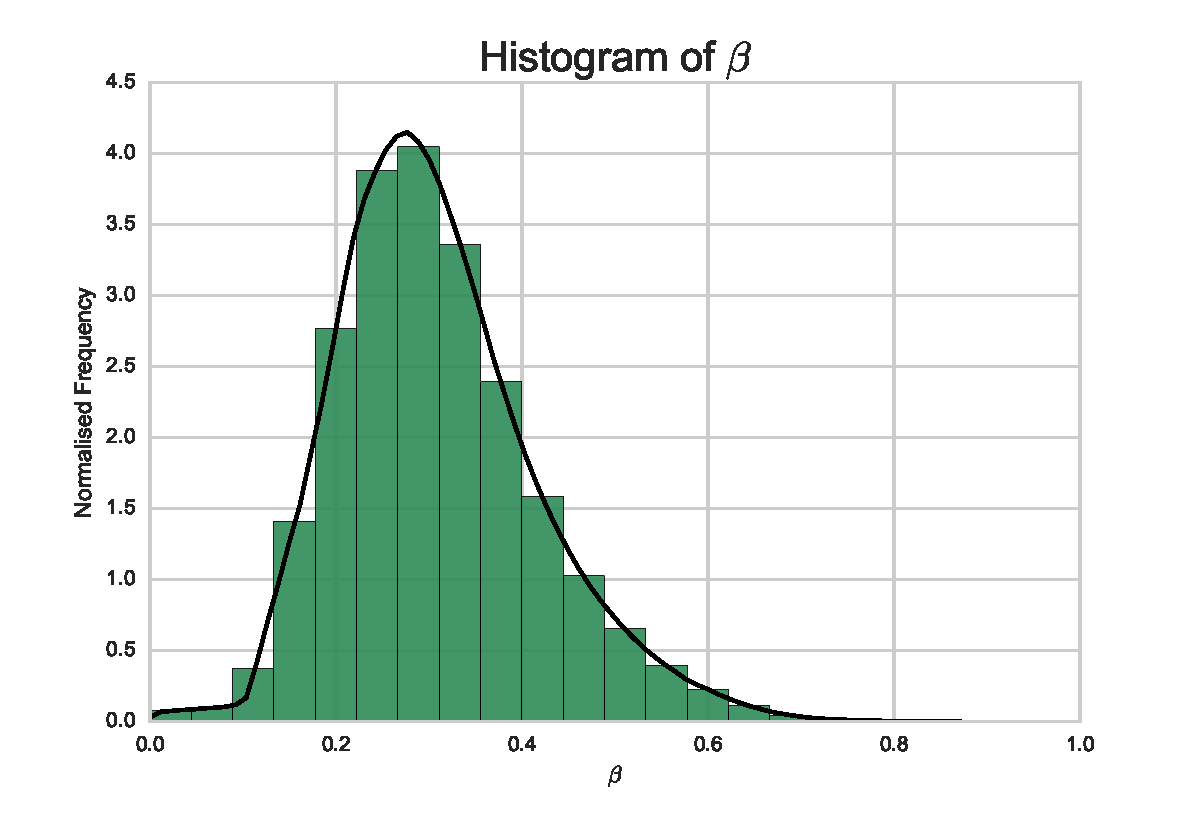
\includegraphics[width=0.5\textwidth]{images/ratio_actual_bound}
  \end{center}
  \caption{Normalised histogram of $E$, with estimated pdf.}
  \label{fig:bound_ratio_hist}
\end{figure}

Recalling Section ? Let $p_{(-1)}$, $p_{(-2)}$ and $p_{(-3)}$ denoted the
probabilities of $\Omega$ reaching deadlocked state (-1), (-2) and (-3)
respectively, calculated using Equation~\ref{eq:abs_probs}.

Figures~\ref{fig:scatter_p1} and \ref{fig:scatter_p3} show scatter plots of
$p_{(-1)}$ and $p_{(-3)}$ against the ratio $E$ respectively (each taking a
random sample of 100000 data points for ease of graphing).  It can be seen that
$p_{(-3)}$ has a strong affect on the tightness of the bound, as the probability
of reaching deadlocked state (-3) increases, the bound becomes tighter.  This
effect seems to only begin as the probability increases above $p_{(-3)}
\approx 0.175$.

% The sentence below is not well written at all.
Queueing networks with absorption probability $p_{(-3)} \leq
0.175$ are either unaffected by this effect, or there are more complicated
effects occurring simultaneously to obscure this effect.

The probability of reaching deadlocked state (-1) does not seem to affect the
tightness of the bound.  The same conclusion can be deduced for $p_{(-2)}$ as
the mechanics of the $\Omega$ system are symmetrical.

\begin{figure}[!htbp]
\begin{subfigure}[b]{0.5\textwidth}
  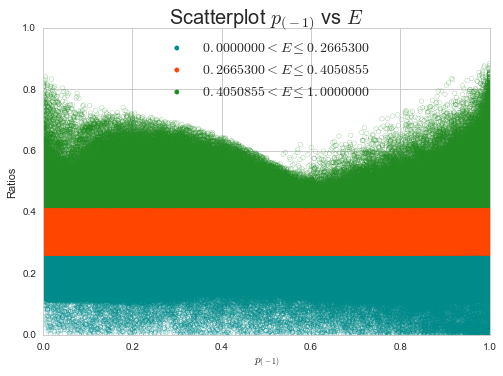
\includegraphics[width=\textwidth]{images/scatter_p1_ratio_p}
  \caption{Scatterplot of $p_{(-1)}$ against $E$.}
  \label{fig:scatter_p1}
\end{subfigure}
\begin{subfigure}[b]{0.5\textwidth}
  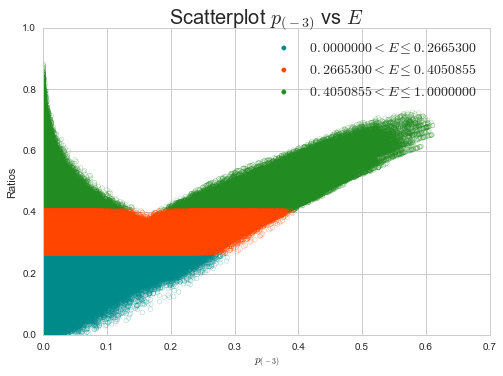
\includegraphics[width=\textwidth]{images/scatter_p3_ratio_p}
  \caption{Scatterplot of $p_{(-3)}$ against $E$.}
  \label{fig:scatter_p3}
\end{subfigure}
\caption{Scatter plots of absorption probabilities against $E$.}
\label{fig:pscatterplot_ratio_analysis}
\end{figure}

This clearly highlights that the assumptions made about the
$\widetilde{\Omega}_{1_1}$ and $\widetilde{\Omega}_{1_2}$ systems in the proof
of Theorem~\ref{thrm:bound} overestimate the difference between
$\widetilde{\omega}_{1_1}$ and $\omega_{1_1}$, and between
$\widetilde{\omega}_{1_2}$ and $\omega_{1_2}$.
% Add a sentence here highlighting the positives and when the bound is good as a
% last sentence.

\section{Conclusions}

This paper, motivated by a gap in the literature, has explored deadlock in open
restricted queueing networks.  It has been shown that analysing a queueing
network's corresponding state digraph is sufficient to detect when deadlock
occurs in queueing network systems.  In general the presence of a knot in the
state digraph will highlight that deadlock has occurred in the network, however
for special cases only the presence of a weakly connected component with no sink
is required.  Incorporating this into a simulation model, time to deadlock could
be recorded.

Markov models of five deadlocking queueing networks were built.  Using linear
algebraic techniques the expected time to deadlock from each state was found,
and its behaviour as system parameters varied explored.  These analytical
results were compared with results obtained from the simulation model.  Finally
a bound on the expected time to deadlock for one of these models was given, that
was found to be tighter for those networks that have high probability of
reaching deadlocked state \((-3)\).

This analysis of deadlock is a contribution to the literature and methodological
understanding of the study of queueing networks.

For the Markov models built in this paper Poisson arrivals and exponential
service rates were assumed.  A future research direction could be to model other
service and arrival distributions using phase-type distributions, and
incorporating these into the Markov models of deadlocking queueing networks.

\bibliographystyle{plain}
\bibliography{refs}

\end{document}
